\documentclass{beamer}

% --- Metropolis theme (modern, minimal) ---
\usetheme{metropolis}
\usepackage{appendixnumberbeamer}

\usepackage{xcolor}
\usepackage{mathrsfs}
\usepackage{amsmath}
\usepackage{amssymb}
\usepackage{bm}
\usepackage{booktabs}
\usepackage{enumitem}
\usepackage{hyperref}
\usepackage{caption}
\usepackage{graphicx}
\usepackage{subcaption}
\usepackage{tikz}
\usetikzlibrary{shapes.geometric, arrows.meta, positioning, fit, backgrounds, decorations.pathmorphing}
\usepackage{tcolorbox}
\tcbuselibrary{skins, breakable}
\captionsetup[figure]{font=tiny}
\graphicspath{{../figures/}}

\usepackage[
    backend=biber,
    style=alphabetic, 
    sorting=ynt
]{biblatex}

% --- Colour palette ---
\definecolor{CSred}{RGB}{160,32,60}
\definecolor{CSgrey}{RGB}{136,121,150}
\definecolor{CSlight}{RGB}{245,240,248}
\definecolor{alertorange}{RGB}{200,80,0} 
\definecolor{metrobg}{RGB}{255,255,255}
\definecolor{greenok}{RGB}{34,120,60}

% --- Metropolis overrides ---
\setbeamercolor{normal text}{fg=black!85, bg=metrobg}
\setbeamercolor{frametitle}{bg=CSred, fg=white}
\setbeamercolor{title separator}{fg=CSred}
\setbeamercolor{progress bar}{fg=CSred, bg=CSgrey!40}
\setbeamercolor{alerted text}{fg=CSred}
\setbeamercolor{block title}{bg=CSred, fg=white}
\setbeamercolor{block body}{bg=CSlight}
\metroset{progressbar=frametitle, sectionpage=none, numbering=fraction}
\setbeamerfont{frametitle}{series=\bfseries, size=\normalsize}

% --- tcolorbox styles ---
\tcbset{
  keybox/.style={
    colback=CSlight, colframe=CSred, fonttitle=\bfseries\small,
    boxrule=0.8pt, arc=3pt, left=5pt, right=5pt, top=4pt, bottom=4pt
  },
  warnbox/.style={
    colback=orange!7, colframe=alertorange, fonttitle=\bfseries\small,
    boxrule=0.8pt, arc=3pt, left=5pt, right=5pt, top=4pt, bottom=4pt
  },
  stressbox/.style={
    colback=CSlight, colframe=CSgrey, fonttitle=\bfseries\footnotesize,
    boxrule=0.8pt, arc=4pt, left=4pt, right=4pt, top=3pt, bottom=3pt
  },
  resultbox/.style={
    colback=green!5, colframe=greenok, fonttitle=\bfseries\small,
    boxrule=0.8pt, arc=3pt, left=5pt, right=5pt, top=4pt, bottom=4pt
  }
}

% --- Title info ---
\title{Inverse Problems and Imaging}
\subtitle{Reverse-Time and Kirchhoff Migration}
\author{Adonis~Jamal \quad Jean-Vincent~Martini}
\institute{\'Ecole Normale Sup\'erieure Paris-Saclay --- MVA 2025-2026}
\date{March 27th, 2026}

\titlegraphic{%
  \hfill
  
\includegraphics[height=1.0cm]{img/logo_ens-ps.png}
  \hspace{0.4cm}
  
\includegraphics[height=1.1cm]{img/logo_mva.jpg}
}

\begin{document}

\maketitle

% ==============================================================================
% SECTION 1: OVERVIEW AND OBJECTIVES
% ==============================================================================

\begin{frame}{Overview and Objectives}
  \footnotesize
  \begin{tcolorbox}[keybox, title=Goal]
    Reconstruct the location of a \textbf{point-like reflector} from time-harmonic or broadband measurement data in 2D, using synthetic array data.
  \end{tcolorbox}
  
    \begin{tcolorbox}[stressbox, title=Configurations studied]
      \footnotesize
      \begin{itemize}\setlength\itemsep{0.1pt}
        \item \textbf{Full aperture:} circular array of transducers.
        \item \textbf{Partial aperture:} linear array of transducers.
        \item \textbf{Broadband:} partial aperture with a time-dependant signal on a frequency band.
        \item \textbf{Noisy:} addition of a Gaussian noise.
      \end{itemize}  
    \end{tcolorbox}

  % TikZ illustration of the imaging setup
  \begin{center}
  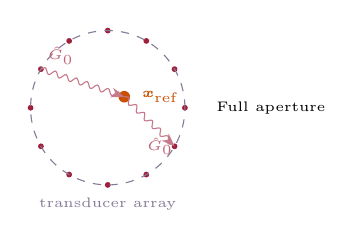
\begin{tikzpicture}[>=Stealth, font=\scriptsize, scale=0.7]
    % Circular array
    \foreach \a in {0,30,...,330}{
      \fill[CSred] ({1.4*cos(\a)},{1.4*sin(\a)}) circle (1.5pt);
    }
    \draw[CSgrey, dashed, thin] (0,0) circle (1.4);
    \node[font=\tiny, CSgrey] at (0,-1.75) {transducer array};
    % Reflector
    \fill[alertorange] (0.3,0.2) circle (3pt);
    \node[font=\tiny, alertorange, right] at (0.45,0.2) {$\bm{x}_{\mathrm{ref}}$};
    % Waves
    \draw[CSred!60, decorate, decoration={snake, amplitude=1pt, segment length=4pt}, ->]
      ({1.4*cos(150)},{1.4*sin(150)}) -- (0.3,0.2);
    \draw[CSred!60, decorate, decoration={snake, amplitude=1pt, segment length=4pt}, ->]
      (0.3,0.2) -- ({1.4*cos(330)},{1.4*sin(330)});
    \node[font=\tiny, CSred!70] at (-0.85,0.95) {$\hat{G}_0$};
    \node[font=\tiny, CSred!70] at (0.95,-0.7) {$\hat{G}_0$};
    % Labels
    \node[font=\tiny, right] at (1.8,0) {Full aperture};
  \end{tikzpicture}
  \hspace{0.8cm}
  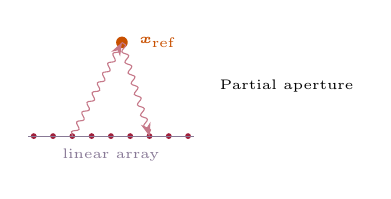
\begin{tikzpicture}[>=Stealth, font=\scriptsize, scale=0.7]
    % Linear array
    \foreach \x in {-1.4,-1.05,...,1.4}{
      \fill[CSred] (\x,-1.2) circle (1.5pt);
    }
    \draw[CSgrey, thin] (-1.5,-1.2) -- (1.5,-1.2);
    \node[font=\tiny, CSgrey] at (0,-1.55) {linear array};
    % Reflector
    \fill[alertorange] (0.2,0.5) circle (3pt);
    \node[font=\tiny, alertorange, right] at (0.35,0.5) {$\bm{x}_{\mathrm{ref}}$};
    % Waves
    \draw[CSred!60, decorate, decoration={snake, amplitude=1pt, segment length=4pt}, ->]
      (-0.7,-1.2) -- (0.2,0.5);
    \draw[CSred!60, decorate, decoration={snake, amplitude=1pt, segment length=4pt}, ->]
      (0.2,0.5) -- (0.7,-1.2);
    \node[font=\tiny, right] at (1.8,-0.3) {Partial aperture};
  \end{tikzpicture}
  \end{center}
\end{frame}


% ==============================================================================
% SECTION 2: THEORETICAL TOOLS
% ==============================================================================

\begin{frame}{Green's Function and Data Model}
  \footnotesize
  \vspace{-0.2cm}
  \begin{tcolorbox}[keybox, title=2D Homogeneous Green's Function]
    Propagation speed $c_0=1$. The Green's function satisfies:
    \vspace{-0.25cm}
    $$\Delta_x \hat{G}_0 + \omega^2 \hat{G}_0 = -\delta(x-y), \quad x \in \mathbb{R}^2$$
    \vspace{-0.45cm}

    with Sommerfeld radiation condition. Explicit solution:
    \vspace{-0.25cm}
    $$\hat{G}_0(\omega, x, y) = \frac{i}{4}\, H_0^{(1)}(\omega |x-y|)$$
    \vspace{-0.45cm}

    {\footnotesize where $H_0^{(1)}(s) = J_0(s) + iY_0(s)$ is the Hankel function of the first kind.}
  \end{tcolorbox}

  \vspace{-0.15cm} 
  \begin{tcolorbox}[stressbox, title=Data Model (Born Approximation)]
    \footnotesize
    For a point reflector at $\bm{x}_{\mathrm{ref}}$, the data entry for receiver $r$ and source $s$:
    \vspace{-0.2cm}
    $$\hat{u}_{rs}(\omega) = \omega^2\, \hat{G}_0(\omega, \bm{x}_r, \bm{x}_{\mathrm{ref}})\, \hat{G}_0(\omega, \bm{x}_{\mathrm{ref}}, \bm{x}_s)$$
    \vspace{-0.4cm}

    In matrix form (rank-1 structure):
    \vspace{-0.2cm}
    $$\hat{U}(\omega) = -\frac{\omega^2}{16}\, \mathbf{v}\mathbf{v}^T, \quad v_t = H_0^{(1)}\!\bigl(\omega|\bm{x}_t - \bm{x}_{\mathrm{ref}}|\bigr)$$

    \textbf{Intuition:} a wave travels from source $s$ to reflector, then from reflector to receiver $r$. The data matrix captures all pairwise travel times.
  \end{tcolorbox}
\end{frame}

\begin{frame}{Imaging Functionals: RT, KM and MUSIC}
  \small

  \hspace*{-0.45cm}
  \begin{minipage}{\dimexpr\textwidth+0.7cm\relax}
  \setlength{\columnsep}{0.5pt}
  \begin{columns}[T]
  \begin{column}{0.63\textwidth}
    \begin{tcolorbox}[keybox, title=Reverse-Time (RT) Migration, top=2pt, bottom=2pt]
      \footnotesize
      Back-propagate using the \emph{exact} Green's function:
      \vspace{-0.22cm} 
      \begin{equation*}
        \scriptsize
        \begin{aligned}
          \mathcal{I}_{RT}(\bm{x}) = \frac{1}{2\pi}\!\int\!\! d\omega \sum_{r,s} \overline{\hat{G}_0(\omega, \bm{x}, \bm{x}_r)}\,\hat{u}_{rs}(\omega) \overline{\hat{G}_0(\omega, \bm{x}_s, \bm{x})}
        \end{aligned}
      \end{equation*}
    \end{tcolorbox}

    \begin{tcolorbox}[warnbox, title=Kirchhoff Migration (KM), top=2pt, bottom=1pt]
      \footnotesize
      Approximate $\hat{G}_0 \approx e^{i\omega\mathcal{T}}$ (travel-time only):
      \vspace{-0.22cm}
      \begin{equation*}
        \scriptsize
        \begin{aligned}
          \mathcal{I}_{KM}(\bm{x}) = \frac{1}{2\pi}\!\int\!\! d\omega \sum_{r,s} e^{-i\omega|\bm{x}-\bm{x}_r|}\,\hat{u}_{rs}(\omega)\,e^{-i\omega|\bm{x}_s - \bm{x}|}
        \end{aligned}
      \end{equation*}
    \end{tcolorbox}

    \begin{tcolorbox}[resultbox, title=MUSIC (Signal-Subspace Projection), top=1pt, bottom=2pt]
      \footnotesize
      Project onto the signal subspace:
      \vspace{-0.15cm}
      {\scriptsize\[\mathcal{I}_{MU}(\bm{x}) = |\langle \hat{g}(\omega, \bm{x}),\, v_1 \rangle|^2\]\vspace{-0.5em}}
      {\scriptsize where $\hat{g} = (\hat{G}_0(\omega, \bm{x}, x_r))_{r=1,\dots,N}$, $v_1$: first singular vector of $\hat{U}$.}
    \end{tcolorbox}
  \end{column}

  \begin{column}{0.37\textwidth}
    \begin{tcolorbox}[keybox, title=, top=2pt, bottom=2pt]
      \scriptsize
      \textcolor{greenok}{\textbf{+}} Physically exact\\
      \textcolor{greenok}{\textbf{+}} Robust to noise (coherent averaging)\\
      \textcolor{CSred}{\textbf{--}} Requires exact $\hat{G}_0$ (costly)\\
      \textcolor{CSred}{\textbf{--}} More costly than KM
    \end{tcolorbox}


    \begin{tcolorbox}[warnbox, title=, top=2pt, bottom=2pt] 
      \scriptsize
      \textcolor{greenok}{\textbf{+}} Computationally cheap\\
      \textcolor{greenok}{\textbf{+}} Similar output to RT\\
      \textcolor{CSred}{\textbf{--}} Drops amplitude information\\
      \textcolor{CSred}{\textbf{--}} Fails in complex media
    \end{tcolorbox}

    \begin{tcolorbox}[resultbox, title=, top=2pt, bottom=2pt]
      \scriptsize
      \textcolor{greenok}{\textbf{+}} Super resolution at low noise\\
      \textcolor{greenok}{\textbf{+}} Exploits rank-1 structure\\
      \textcolor{CSred}{\textbf{--}} Fragile beyond noise threshold\\
      \textcolor{CSred}{\textbf{--}} Requires rank-1 assumption
    \end{tcolorbox}
  \end{column}
  \end{columns} 
  \end{minipage} 
\end{frame}

\begin{frame}{Theoretical Focal Spots -- Full Aperture}
  \small
  \vspace{-0.1cm}
  \begin{columns}
  \begin{column}{0.35\textwidth}
    \begin{center}
    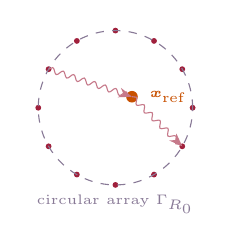
\begin{tikzpicture}[>=Stealth, font=\scriptsize, scale=0.7]
      % Circular array
      \foreach \a in {0,30,...,330}{
        \fill[CSred] ({1.4*cos(\a)},{1.4*sin(\a)}) circle (1.5pt);
      }
      \draw[CSgrey, dashed, thin] (0,0) circle (1.4);
      \node[font=\tiny, CSgrey] at (0,-1.75) {circular array $\Gamma_{R_0}$};
      % Reflector
      \fill[alertorange] (0.3,0.2) circle (3pt);
      \node[font=\tiny, alertorange, right] at (0.45,0.2) {$\bm{x}_{\mathrm{ref}}$};
      % Waves
      \draw[CSred!60, decorate, decoration={snake, amplitude=1pt, segment length=4pt}, ->]
        ({1.4*cos(150)},{1.4*sin(150)}) -- (0.3,0.2);
      \draw[CSred!60, decorate, decoration={snake, amplitude=1pt, segment length=4pt}, ->]
        (0.3,0.2) -- ({1.4*cos(330)},{1.4*sin(330)});
    \end{tikzpicture}
    \end{center}
  \end{column}

  \begin{column}{0.63\textwidth}
    \begin{tcolorbox}[keybox, title=Derivation, top=2pt, bottom=2pt]
      \scriptsize
      As $N\!\to\!\infty$, the sum becomes an integral over $\Gamma_{R_0}$:
      $$\mathcal{I}(\bm{x})\propto
      \left|\!\int_{\Gamma_{R_0}}\!\!
      \overline{H_0^{(1)}\!\big(\omega|\bm{x}\!-\!\bm{y}|\big)}\,
      H_0^{(1)}\!\big(\omega|\bm{x}_{\mathrm{ref}}\!-\!\bm{y}|\big)
      \,d\sigma(\bm{y})\right|^2$$

      Far-field ($R_0\!\gg\!1$): phase difference $\approx \hat{\bm{y}}\cdot(\bm{x}-\bm{x}_{\mathrm{ref}})$.
    \end{tcolorbox}
  \end{column}
  \end{columns}

  \begin{tcolorbox}[stressbox, top=2pt, bottom=2pt]
    \scriptsize
    With $\bm{y}=R_0(\cos\theta,\sin\theta)$ and $\Delta\bm{x}=\bm{x}-\bm{x}_{\mathrm{ref}}$, the angular integral yields:
    \vspace{-0.1cm}
    $$\int_0^{2\pi}\!\! e^{i\omega\hat{\bm{y}}\cdot\Delta\bm{x}}\,d\theta
    = 2\pi\, J_0(\omega|\Delta\bm{x}|)$$
  \end{tcolorbox}

  \begin{tcolorbox}[resultbox, title=Isotropic focal spot]
    \footnotesize
    $$\boxed{\;\mathcal{I}(\bm{x}) \;\sim\; J_0^2\!\bigl(\omega|\bm{x}-\bm{x}_{\mathrm{ref}}|\bigr)\;}$$
    \vspace{-0.1cm}

    {\scriptsize Resolution $\sim\lambda/2$ in all directions (diffraction limit).}
  \end{tcolorbox}
\end{frame}

\begin{frame}{Theoretical Focal Spots -- Partial Aperture}
  \small
  \vspace{-0.2cm}
  \begin{columns}
  \begin{column}{0.38\textwidth}
    \begin{center}
    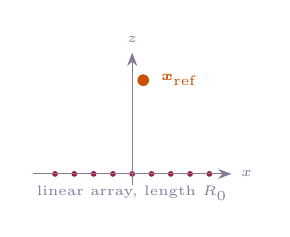
\begin{tikzpicture}[>=Stealth, font=\scriptsize, scale=0.7]
      % Linear array
      \foreach \x in {-1.4,-1.05,...,1.4}{
        \fill[CSred] (\x,-1.2) circle (1.5pt);
      }
      \draw[CSgrey, thin] (-1.5,-1.2) -- (1.5,-1.2);
      \node[font=\tiny, CSgrey] at (0,-1.55) {linear array, length $R_0$};
      % Reflector
      \fill[alertorange] (0.2,0.5) circle (3pt);
      \node[font=\tiny, alertorange, right] at (0.35,0.5) {$\bm{x}_{\mathrm{ref}}$};
      % Axes
      \draw[->, thin, CSgrey] (-1.8,-1.2) -- (1.8,-1.2) node[right, font=\tiny]{$x$};
      \draw[->, thin, CSgrey] (0,-1.4) -- (0,1.0) node[above, font=\tiny]{$z$};
    \end{tikzpicture}
    \end{center}
  \end{column}
  \begin{column}{0.60\textwidth}
    \begin{tcolorbox}[keybox, title=Anisotropic resolution, top=2pt, bottom=2pt]
      \scriptsize
      The limited aperture breaks symmetry $\Rightarrow$ resolution differs in cross-range ($x$) and range ($z$).
    \end{tcolorbox} 
  \end{column}
  \end{columns}

  \vspace{-0.05cm}
  \noindent
  \begin{minipage}[t]{0.48\textwidth}
    \begin{tcolorbox}[stressbox, title=Cross-range ($x$), top=2pt, bottom=2pt]
      \scriptsize
      $$\mathcal{I}(x) \sim \operatorname{sinc}^2\!\!\left(\frac{\pi|x-x_{\mathrm{ref}}|}{r_c}\right)$$
      \vspace{-0.25cm}

      with resolution:
      \vspace{-0.1cm}
      $$r_c = \frac{\lambda\,|\bm{x}_{\mathrm{ref}}|}{R_0}$$
    \end{tcolorbox}
  \end{minipage}
  \hfill
  \begin{minipage}[t]{0.48\textwidth}
    \begin{tcolorbox}[stressbox, title=Range ($z$), top=2pt, bottom=2pt]
      \scriptsize
      {\scriptsize\[\mathcal{I}(z) \sim \smash{\left|\int_0^1 e^{-i\frac{\pi}{2}s^2\frac{|z-z_{\mathrm{ref}}|}{r_l}}\,ds\right|^2}\]\vspace{-1.2em}}
      with resolution:
      \vspace{-0.1cm}
      $$r_l = \frac{2\lambda\,|\bm{x}_{\mathrm{ref}}|^2}{R_0^2}$$
    \end{tcolorbox}
  \end{minipage}

  \vspace{-0.05cm}
  \begin{tcolorbox}[warnbox, top=2pt, bottom=2pt]
    \scriptsize
    \textbf{Key difference:} cross-range $r_c \propto R_0^{-1}$ vs.\ range $r_l \propto R_0^{-2}$. Range resolution degrades faster as aperture shrinks. Mirror artifact at $-z_{\mathrm{ref}}$ (array cannot distinguish $z$ from $-z$).
  \end{tcolorbox}
\end{frame}


% ==============================================================================
% SECTION 3: RESULTS -- FULL APERTURE
% ==============================================================================

\begin{frame}{Full Aperture -- RT, KM and Theoretical Focal Spot}
  \small
  \vspace{-0.2cm}
  \begin{tcolorbox}[stressbox, title=Setup]
    \footnotesize $N\!=\!100$ transducers on a circle, $R_0\!=\!100$, $\omega\!=\!2\pi$, $\bm{x}_{\mathrm{ref}}\!=\!(10,20)$.
  \end{tcolorbox}

  \vspace{-0.15cm}
  \begin{columns}
  \begin{column}{0.6\textwidth}
    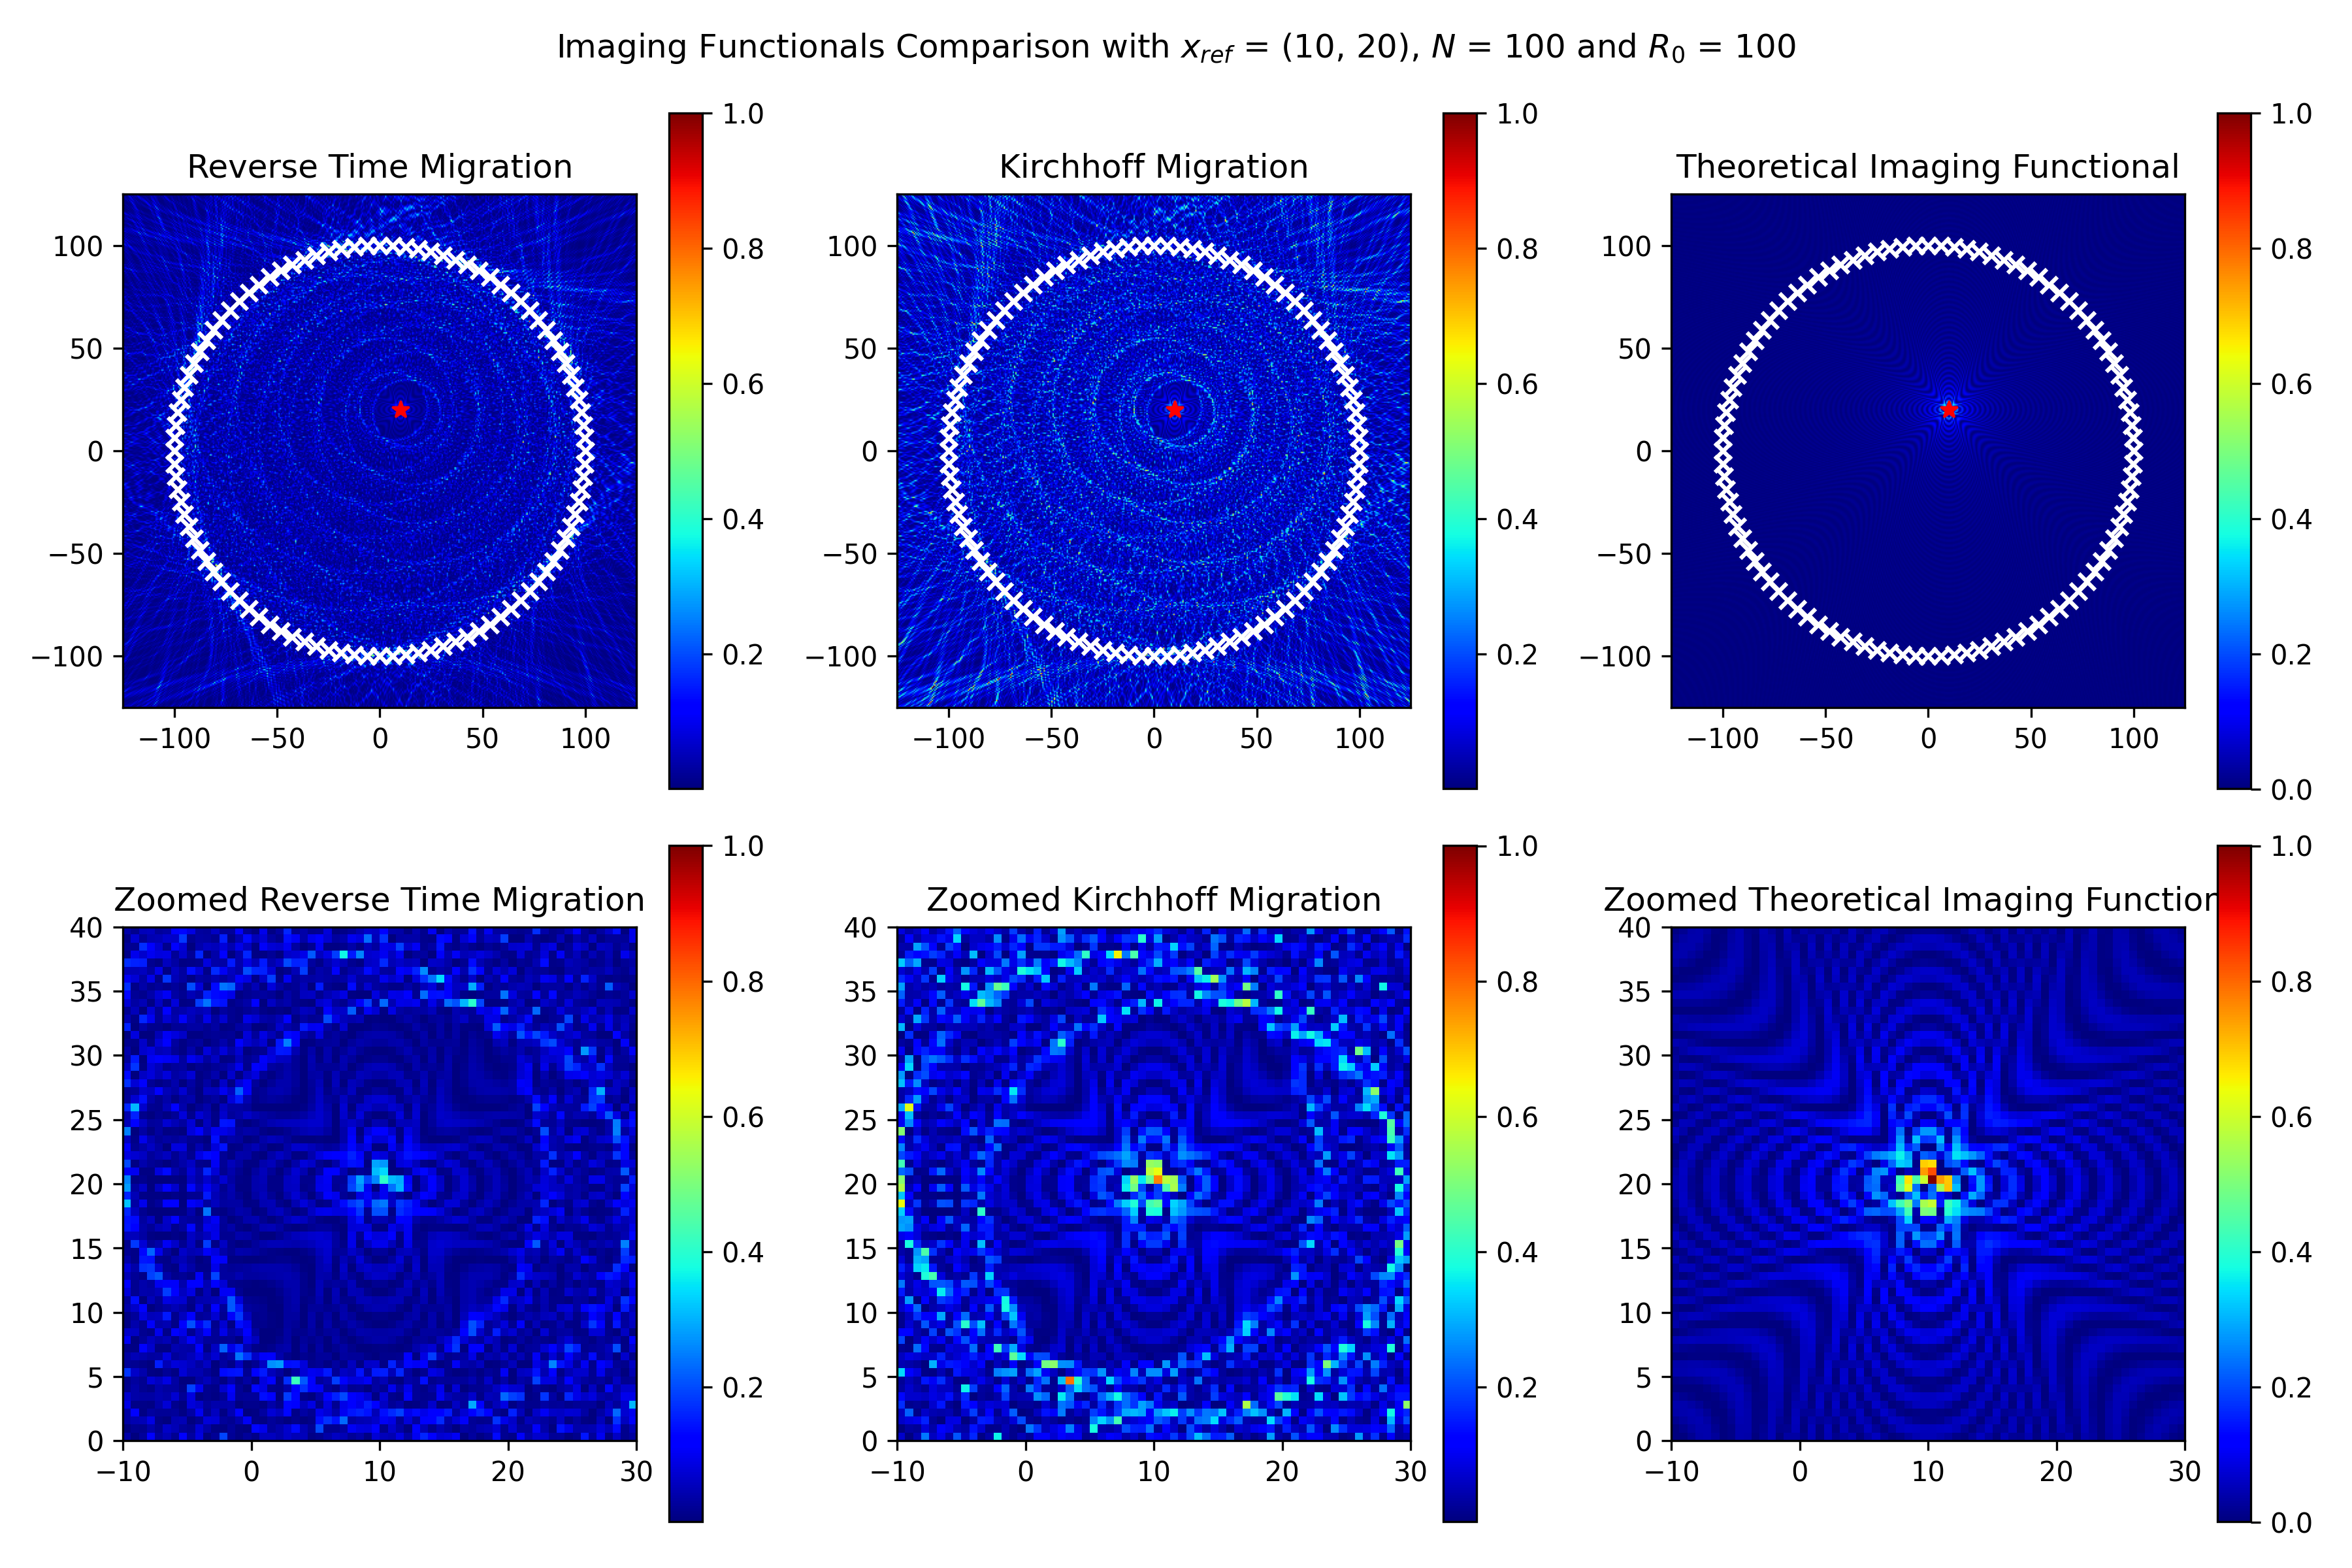
\includegraphics[width=\textwidth]{Full_Aperture.png}
  \end{column}
  \begin{column}{0.38\textwidth}
    \begin{tcolorbox}[keybox, title=Observations]
      \scriptsize
      \begin{itemize}[leftmargin=0.5em, label=\textbullet]\setlength\itemsep{2pt}
        \item RT and KM images are very similar; KM shows minor discrepancies.
        \item Theoretical $J_0^2$ focal spot differs noticeably: derived under $R_0\!\to\!\infty$, $N\!\to\!\infty$.
        \item Near the reflector, all three profiles agree qualitatively despite the missing circular patterns.
      \end{itemize}
    \end{tcolorbox}
  \end{column}
  \end{columns}
\end{frame}

\begin{frame}{Full Aperture -- Multiple Reflector Positions}
  \footnotesize
  \vspace{-0.2cm}
  \begin{tcolorbox}[stressbox, title=Varying reflector position]
    \footnotesize Reflector moved to $(0,0)$, $(0,100)$, $(100,0)$, $(50,50)$, $(40, 80)$.
  \end{tcolorbox}

  \vspace{-0.25cm}
  \begin{center}
    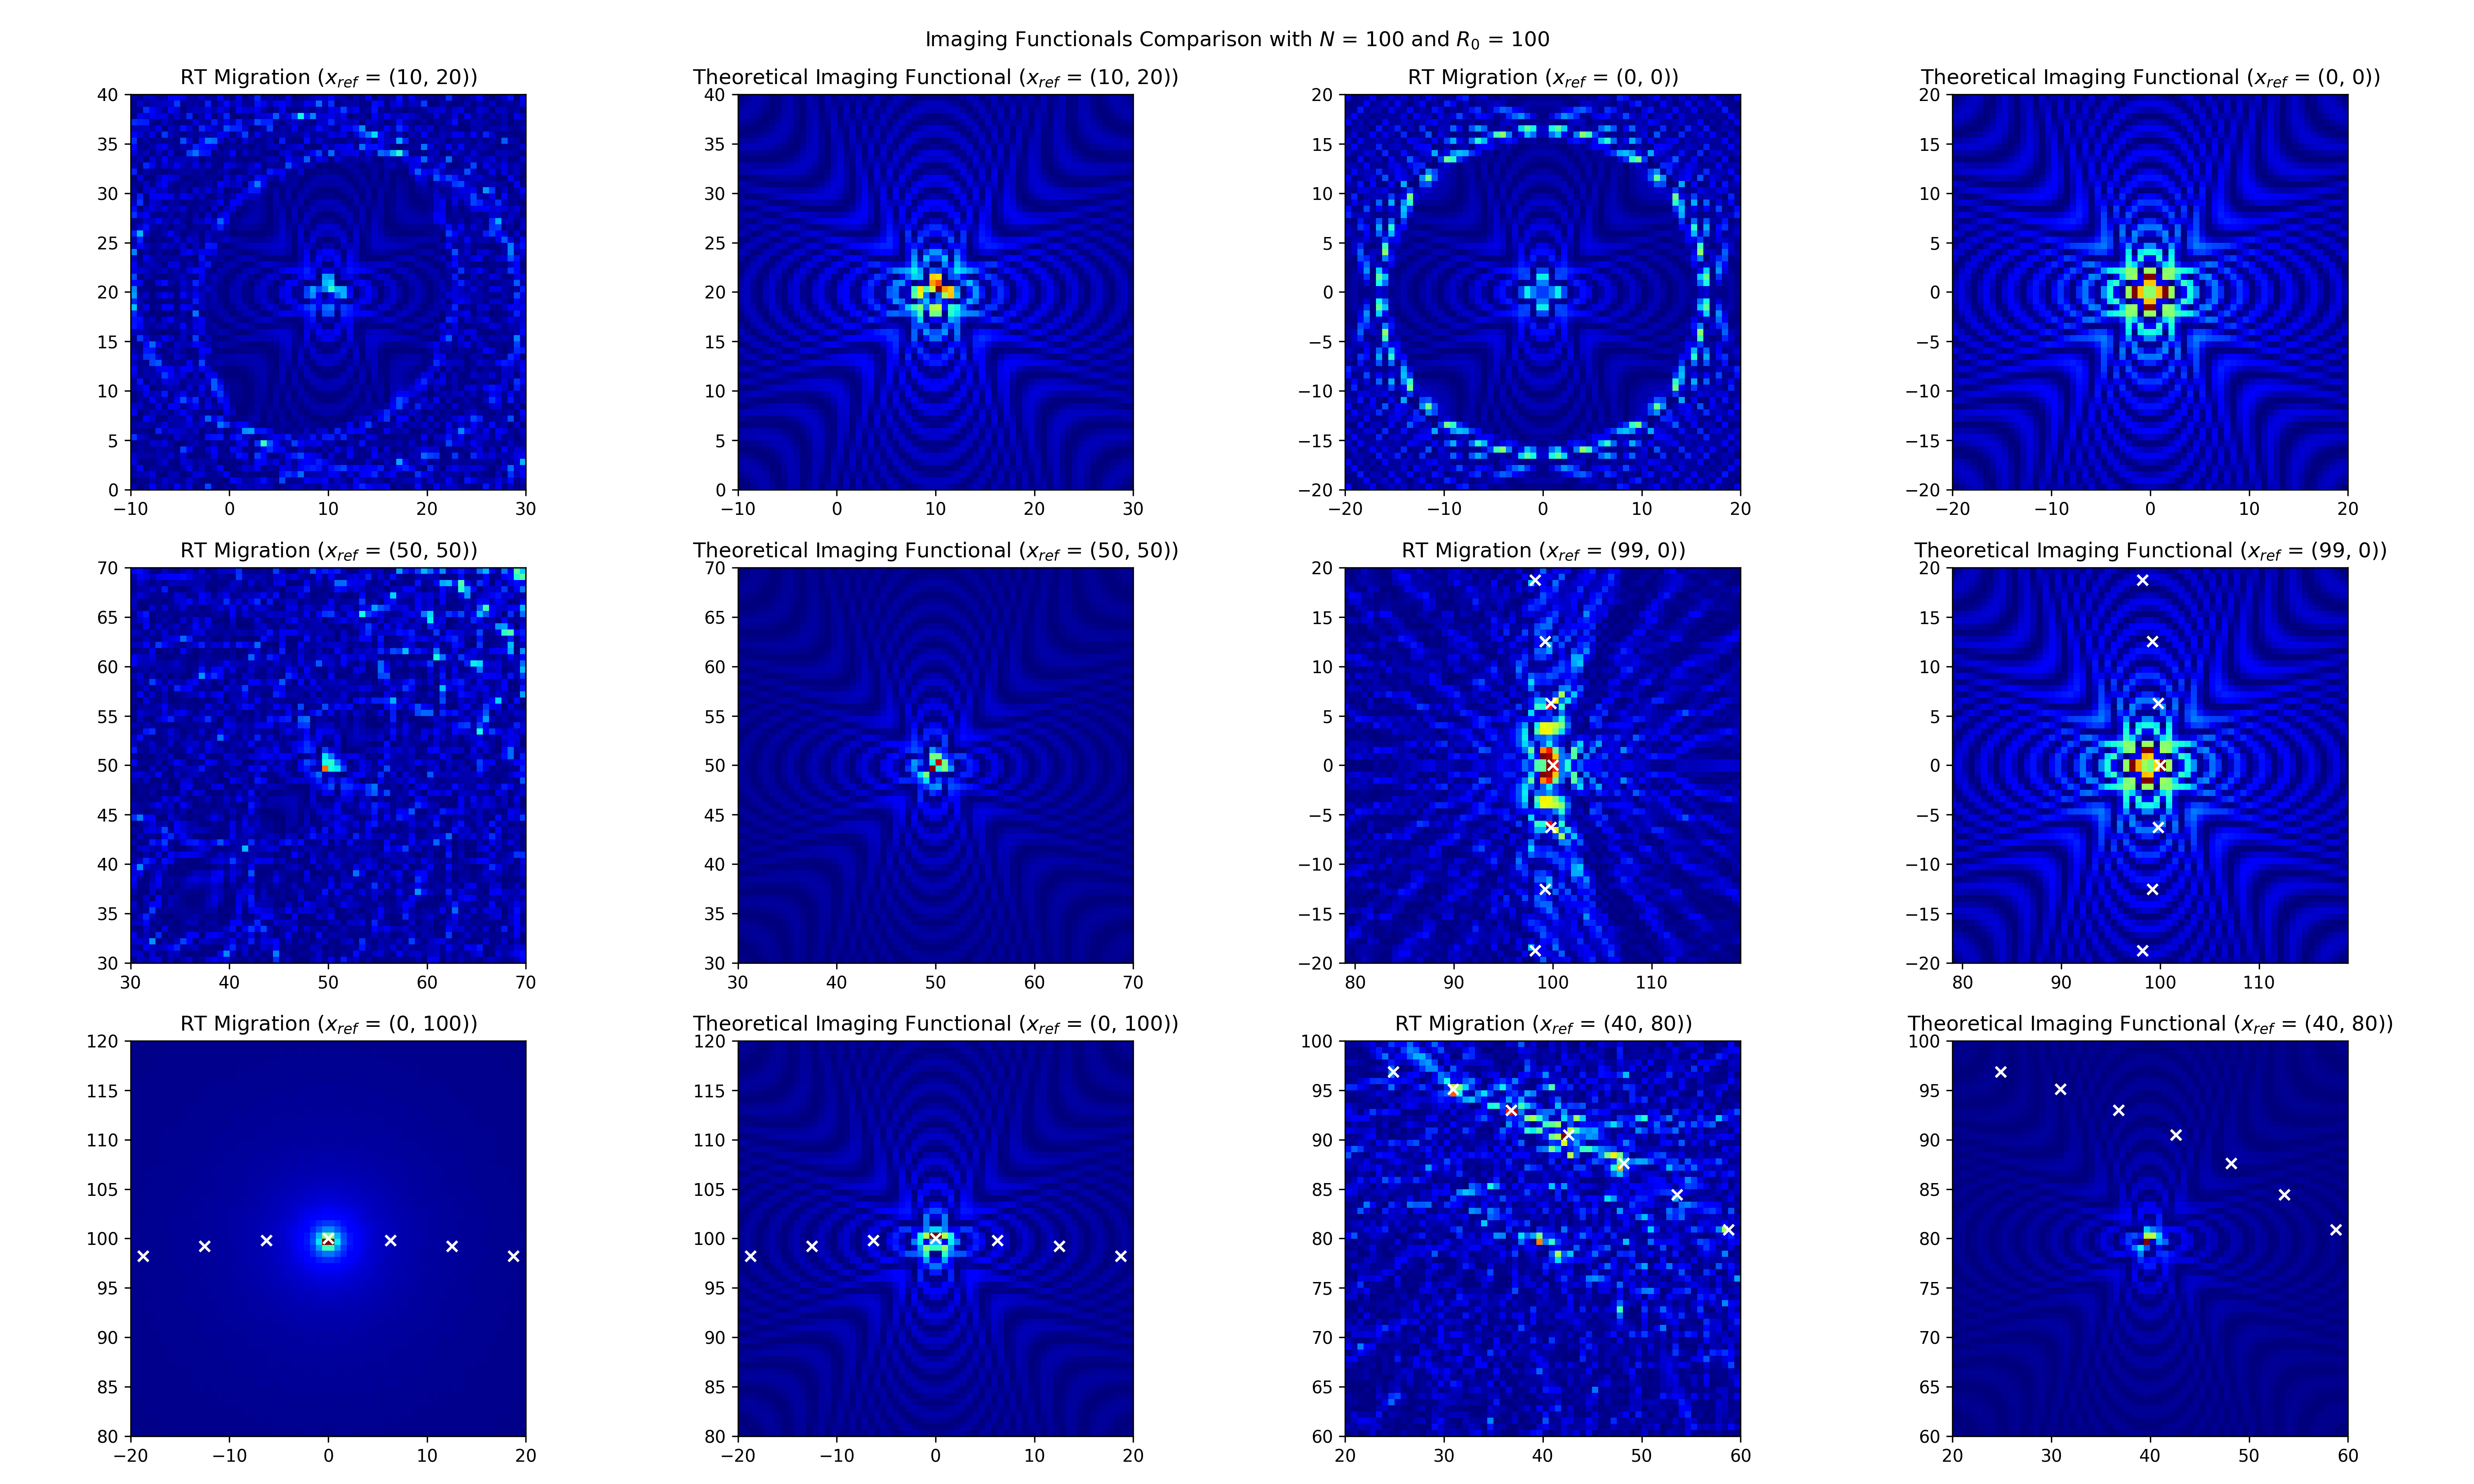
\includegraphics[width=0.78\textwidth]{Full_Aperture_Multiple_Reflectors.png}
  \end{center}

  \vspace{-0.25cm}
  \begin{tcolorbox}[warnbox]
    \footnotesize As the reflector approaches the array boundary, asymptotic assumptions break down $\Rightarrow$ increased discrepancy between RT/KM and the theoretical $J_0^2$ profile.
  \end{tcolorbox}
\end{frame}

\begin{frame}{Full Aperture -- Far-Field Regime}
  \small
  \vspace{-0.2cm}
  \begin{tcolorbox}[stressbox, title=Far-field configuration]
    \footnotesize $R_0 = 1000$, $N = 2000$: pushing toward the asymptotic limit.
  \end{tcolorbox}

  \vspace{-0.15cm}
  \begin{center}
    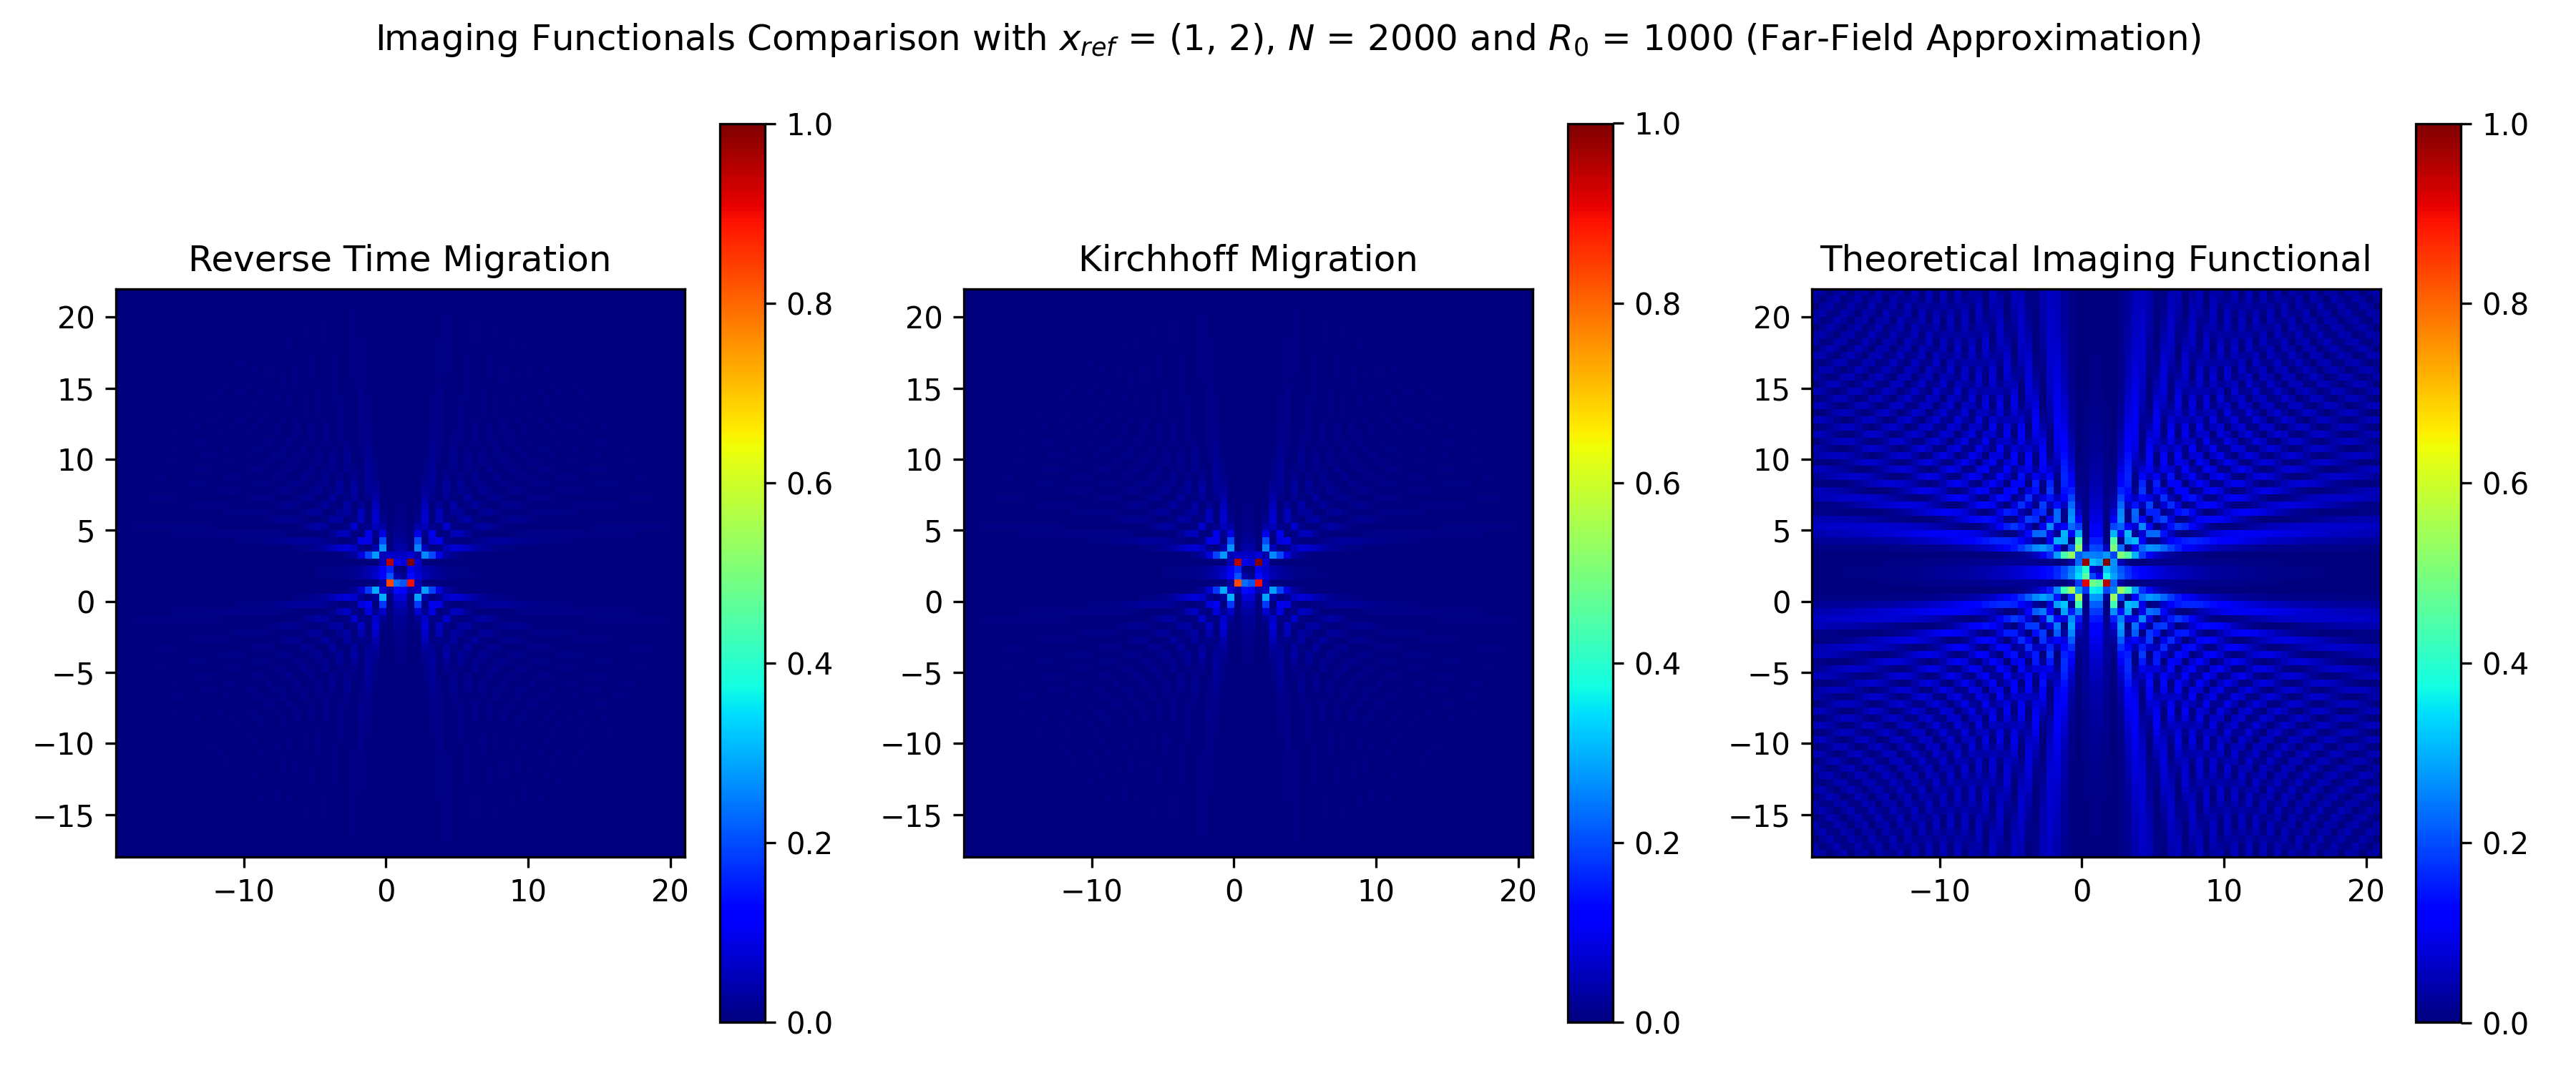
\includegraphics[width=0.8\textwidth]{Full_Aperture_Far_Field.png}
  \end{center}

  \vspace{-0.2cm}
  \begin{tcolorbox}[resultbox, title=Validation]
    \footnotesize With a much larger array and many more transducers, RT and KM \textbf{converge closely} to the theoretical $J_0^2$ focal spot, confirming the validity of the asymptotic formula.
  \end{tcolorbox}
\end{frame}


% ==============================================================================
% SECTION 4: RESULTS -- PARTIAL APERTURE
% ==============================================================================

\begin{frame}{Partial Aperture -- RT, KM and MUSIC}
  \footnotesize
  \vspace{-0.2cm}
  \begin{tcolorbox}[stressbox, title=Setup]
    \footnotesize $N\!=\!100$ transducers on a linear array, $R_0\!=\!100$, $\omega\!=\!2\pi$, $\bm{x}_{\mathrm{ref}}\!=\!(10,20)$.
  \end{tcolorbox}


  \begin{columns} 
  \begin{column}{0.62\textwidth}
    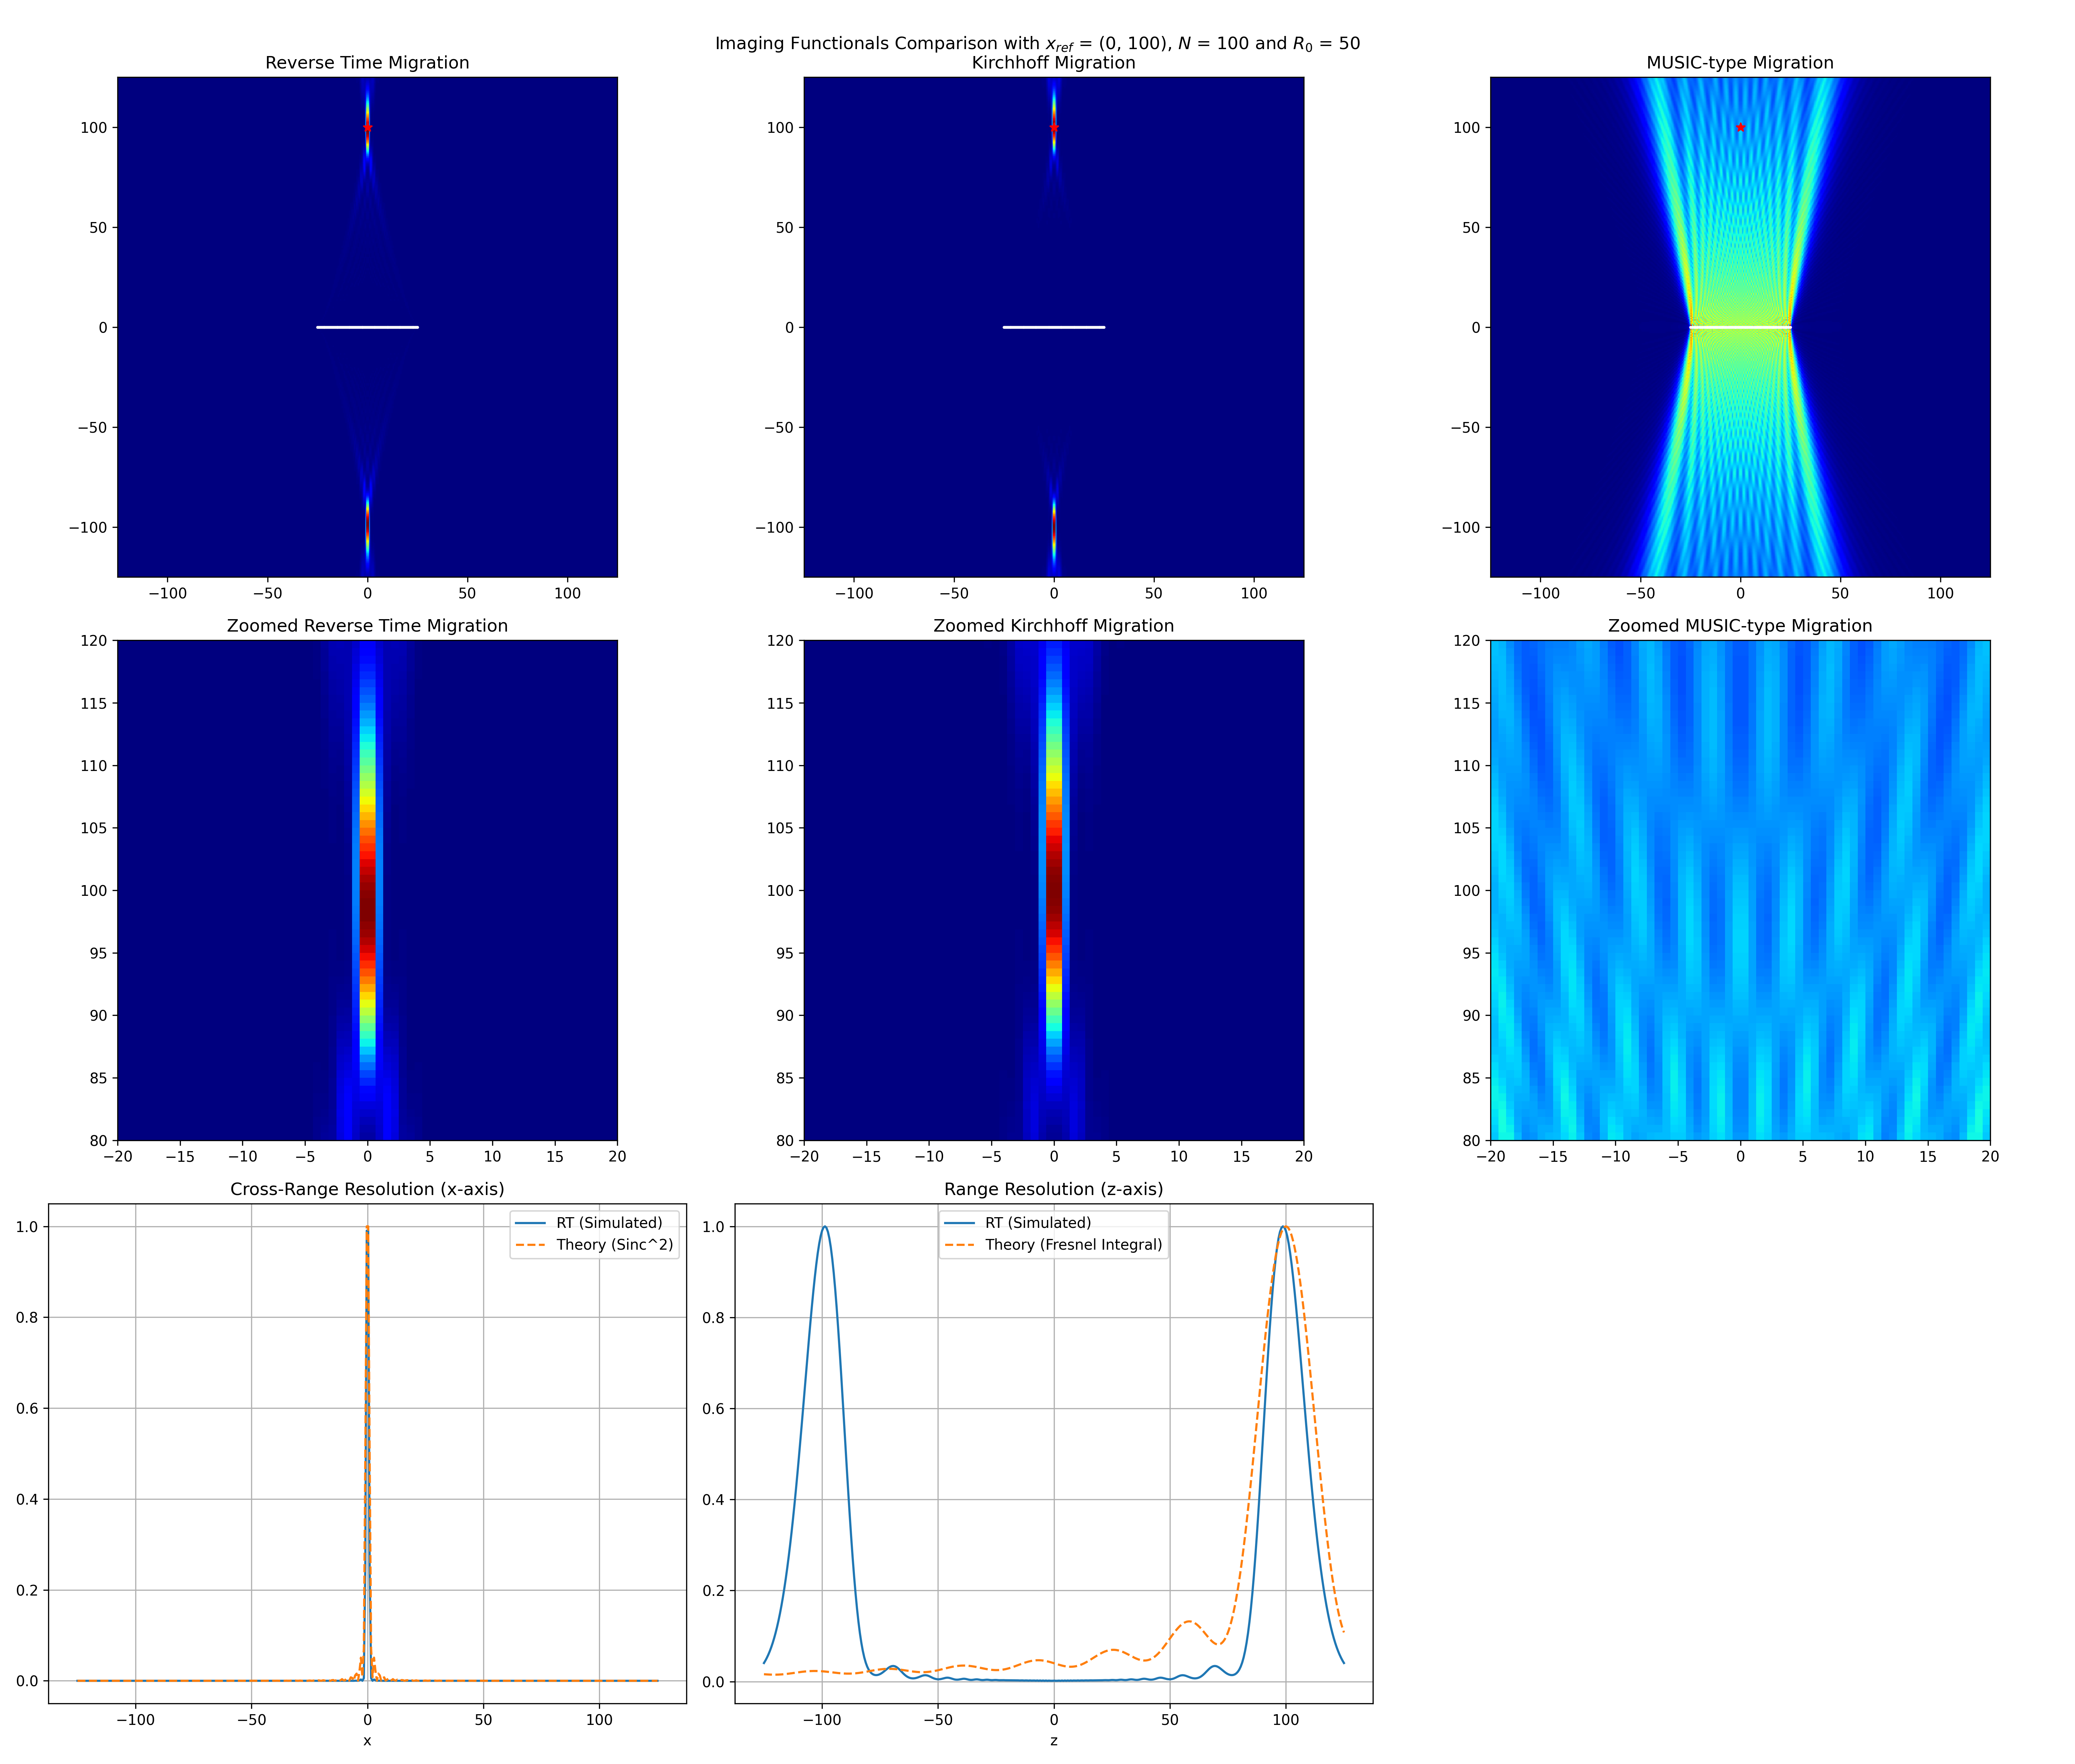
\includegraphics[width=\textwidth]{Partial_Aperture.png}
  \end{column}
  \begin{column}{0.36\textwidth}
    \begin{tcolorbox}[keybox, title=Observations]
      \scriptsize
      \begin{itemize}[leftmargin=0.5em, label=\textbullet]\setlength\itemsep{2pt}
        \item RT, KM and MUSIC closely resemble each other.
        \item \textbf{Cross-range ($x$):} RT reproduces the main peak and secondary lobes.
        \item \textbf{Range ($z$):} a \alert{mirror image} appears at $-z_{\mathrm{ref}}$ (linear geometry cannot distinguish $z$ from $-z$).
      \end{itemize}
    \end{tcolorbox}
  \end{column}
  \end{columns}
\end{frame}

\begin{frame}{Partial Aperture -- Influence of Array Length $R_0$}
  \small
  \vspace{-0.2cm}
  \begin{columns}
  \begin{column}{0.54\textwidth}
    \begin{center}
      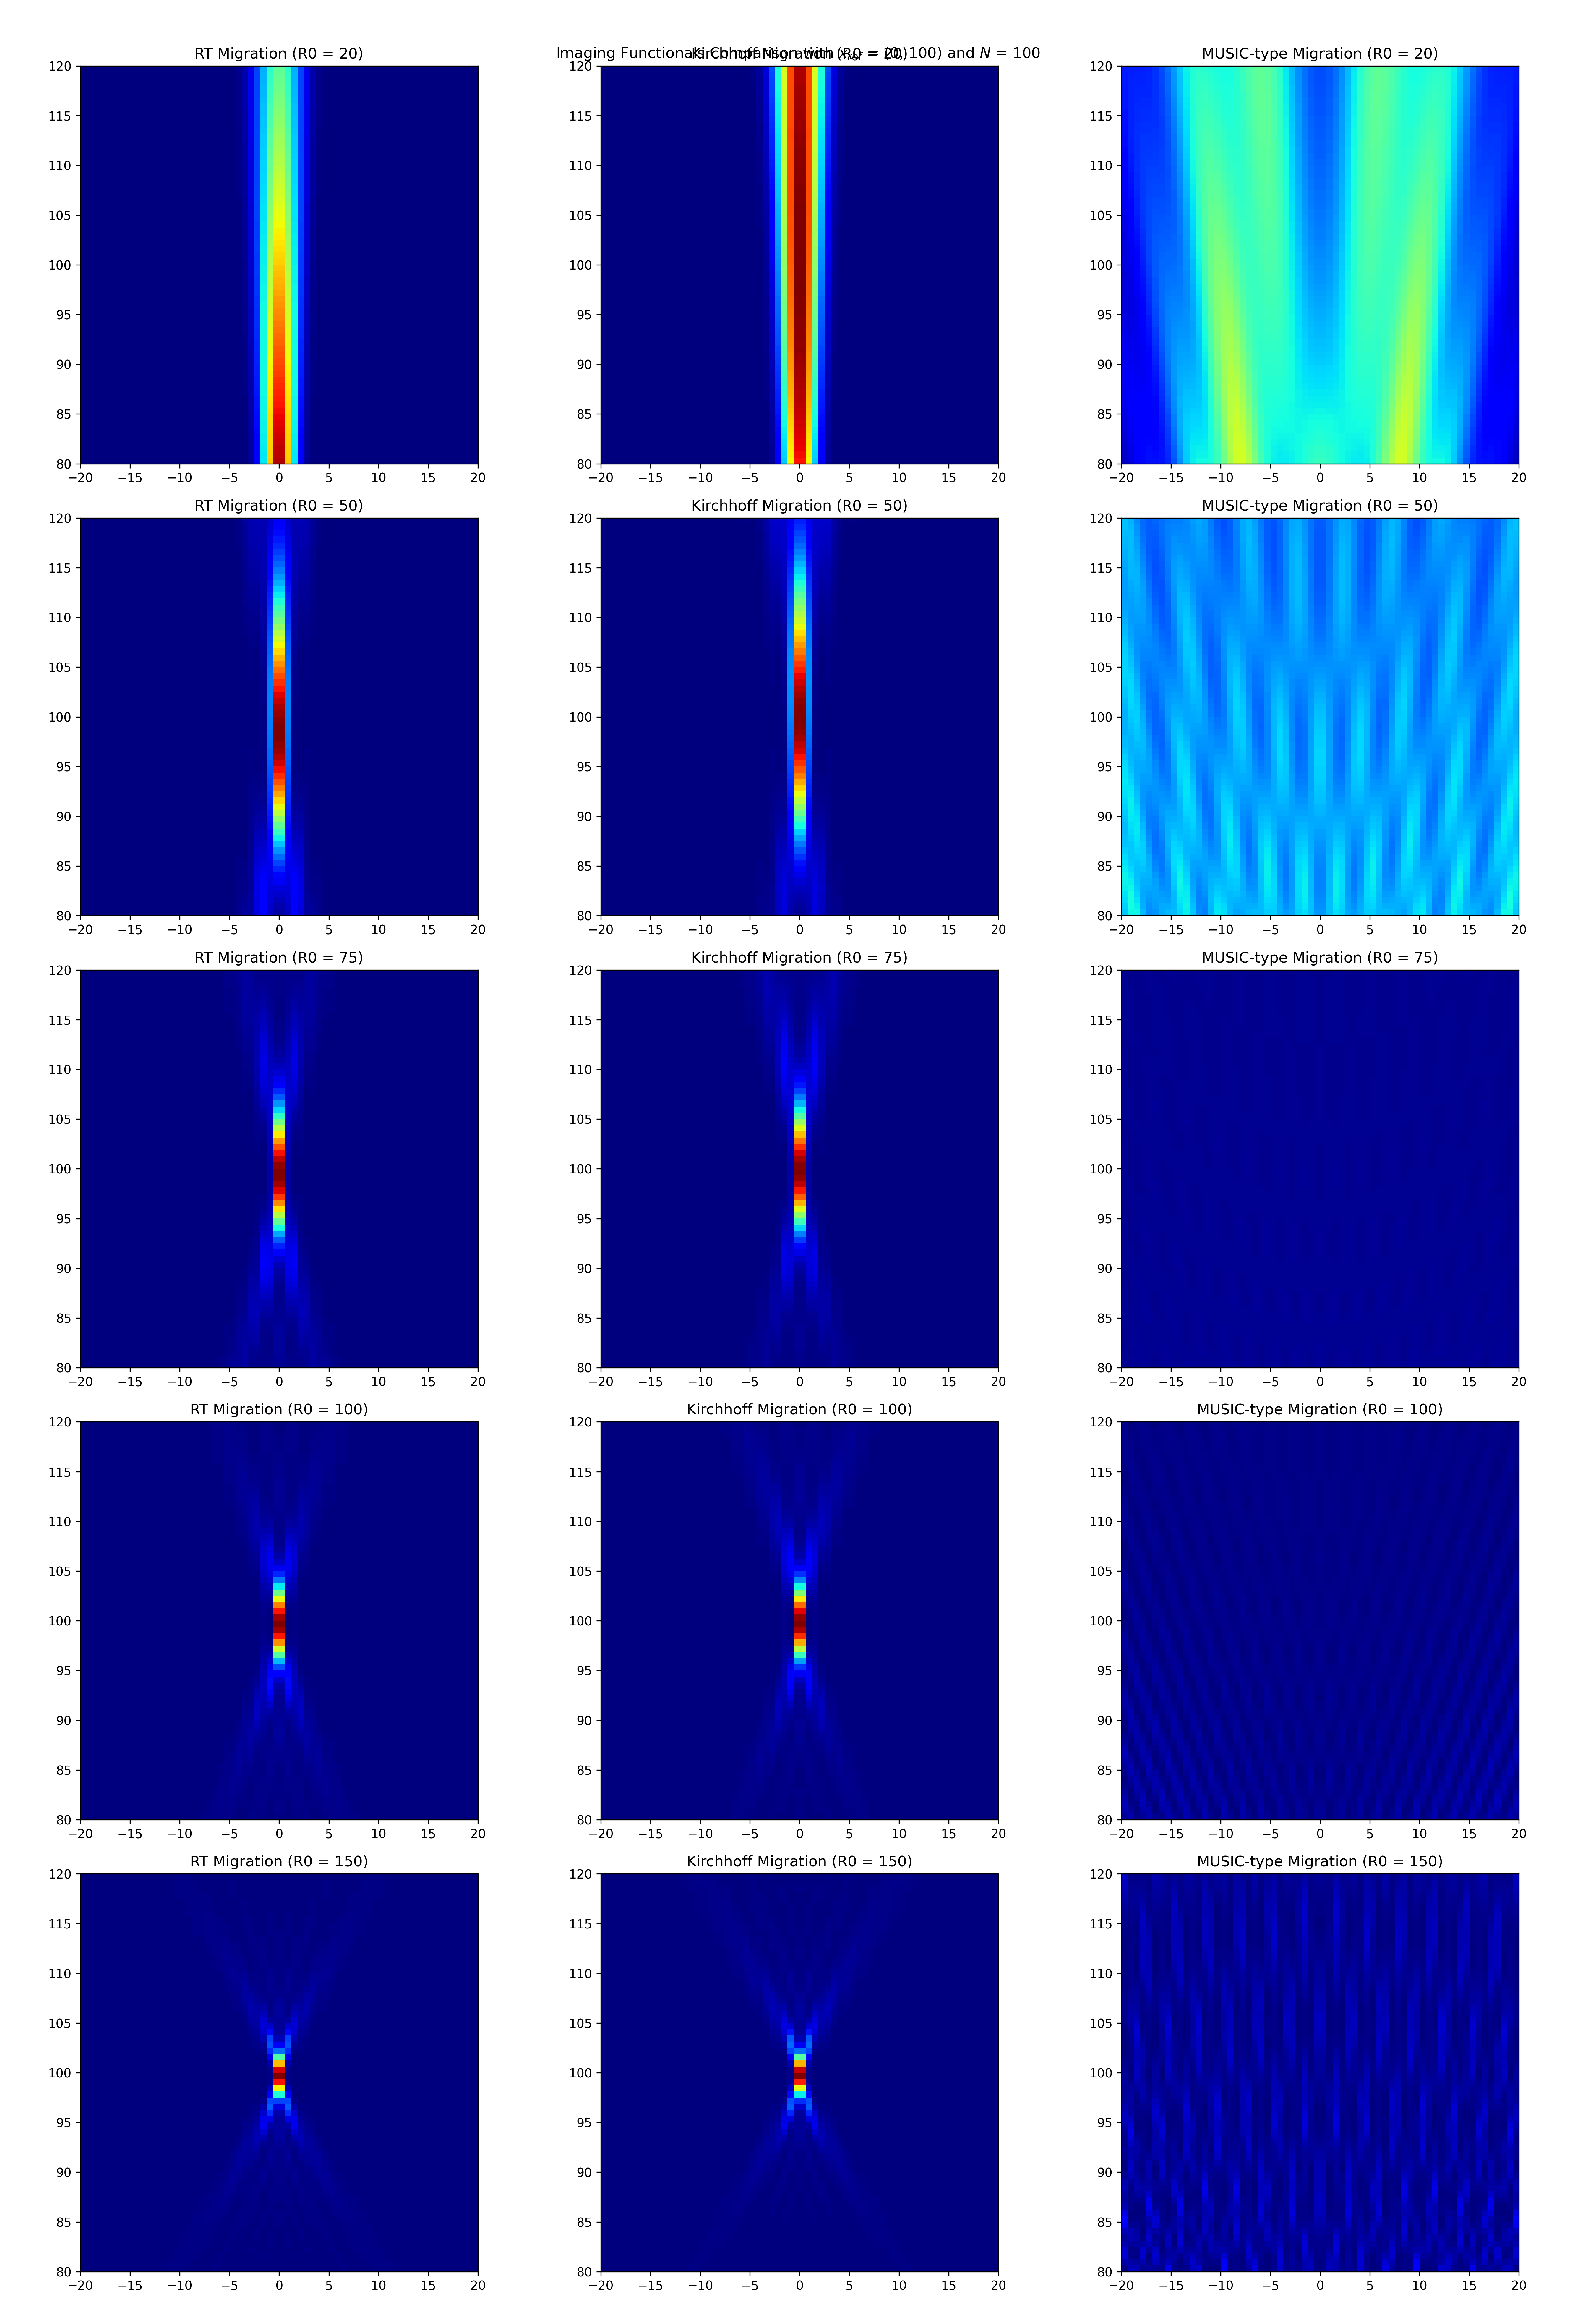
\includegraphics[width=\textwidth]{Partial_Aperture_Multiple_R0.png}
    \end{center}
  \end{column}
  \begin{column}{0.44\textwidth}
    \begin{tcolorbox}[keybox, title=Cross-range resolution]
      \footnotesize
      $$r_c = \frac{\lambda\,|\bm{x}_{\mathrm{ref}}|}{R_0}$$
      Smaller aperture $R_0$ $\Rightarrow$ coarser cross-range resolution.
    \end{tcolorbox}

    \vspace{0.1cm}
    \begin{tcolorbox}[stressbox, title=Key insight]
      \scriptsize As $R_0$ \textbf{increases}, the focal spot \textbf{narrows} in the cross-range direction, consistent with the theoretical $\operatorname{sinc}^2$ prediction.
    \end{tcolorbox}
  \end{column}
  \end{columns}
\end{frame}

\begin{frame}{Partial Aperture -- Multiple Reflector Positions}
  \small
  \vspace{-0.2cm}
  \begin{columns}
  \begin{column}{0.54\textwidth}
    \begin{center}
      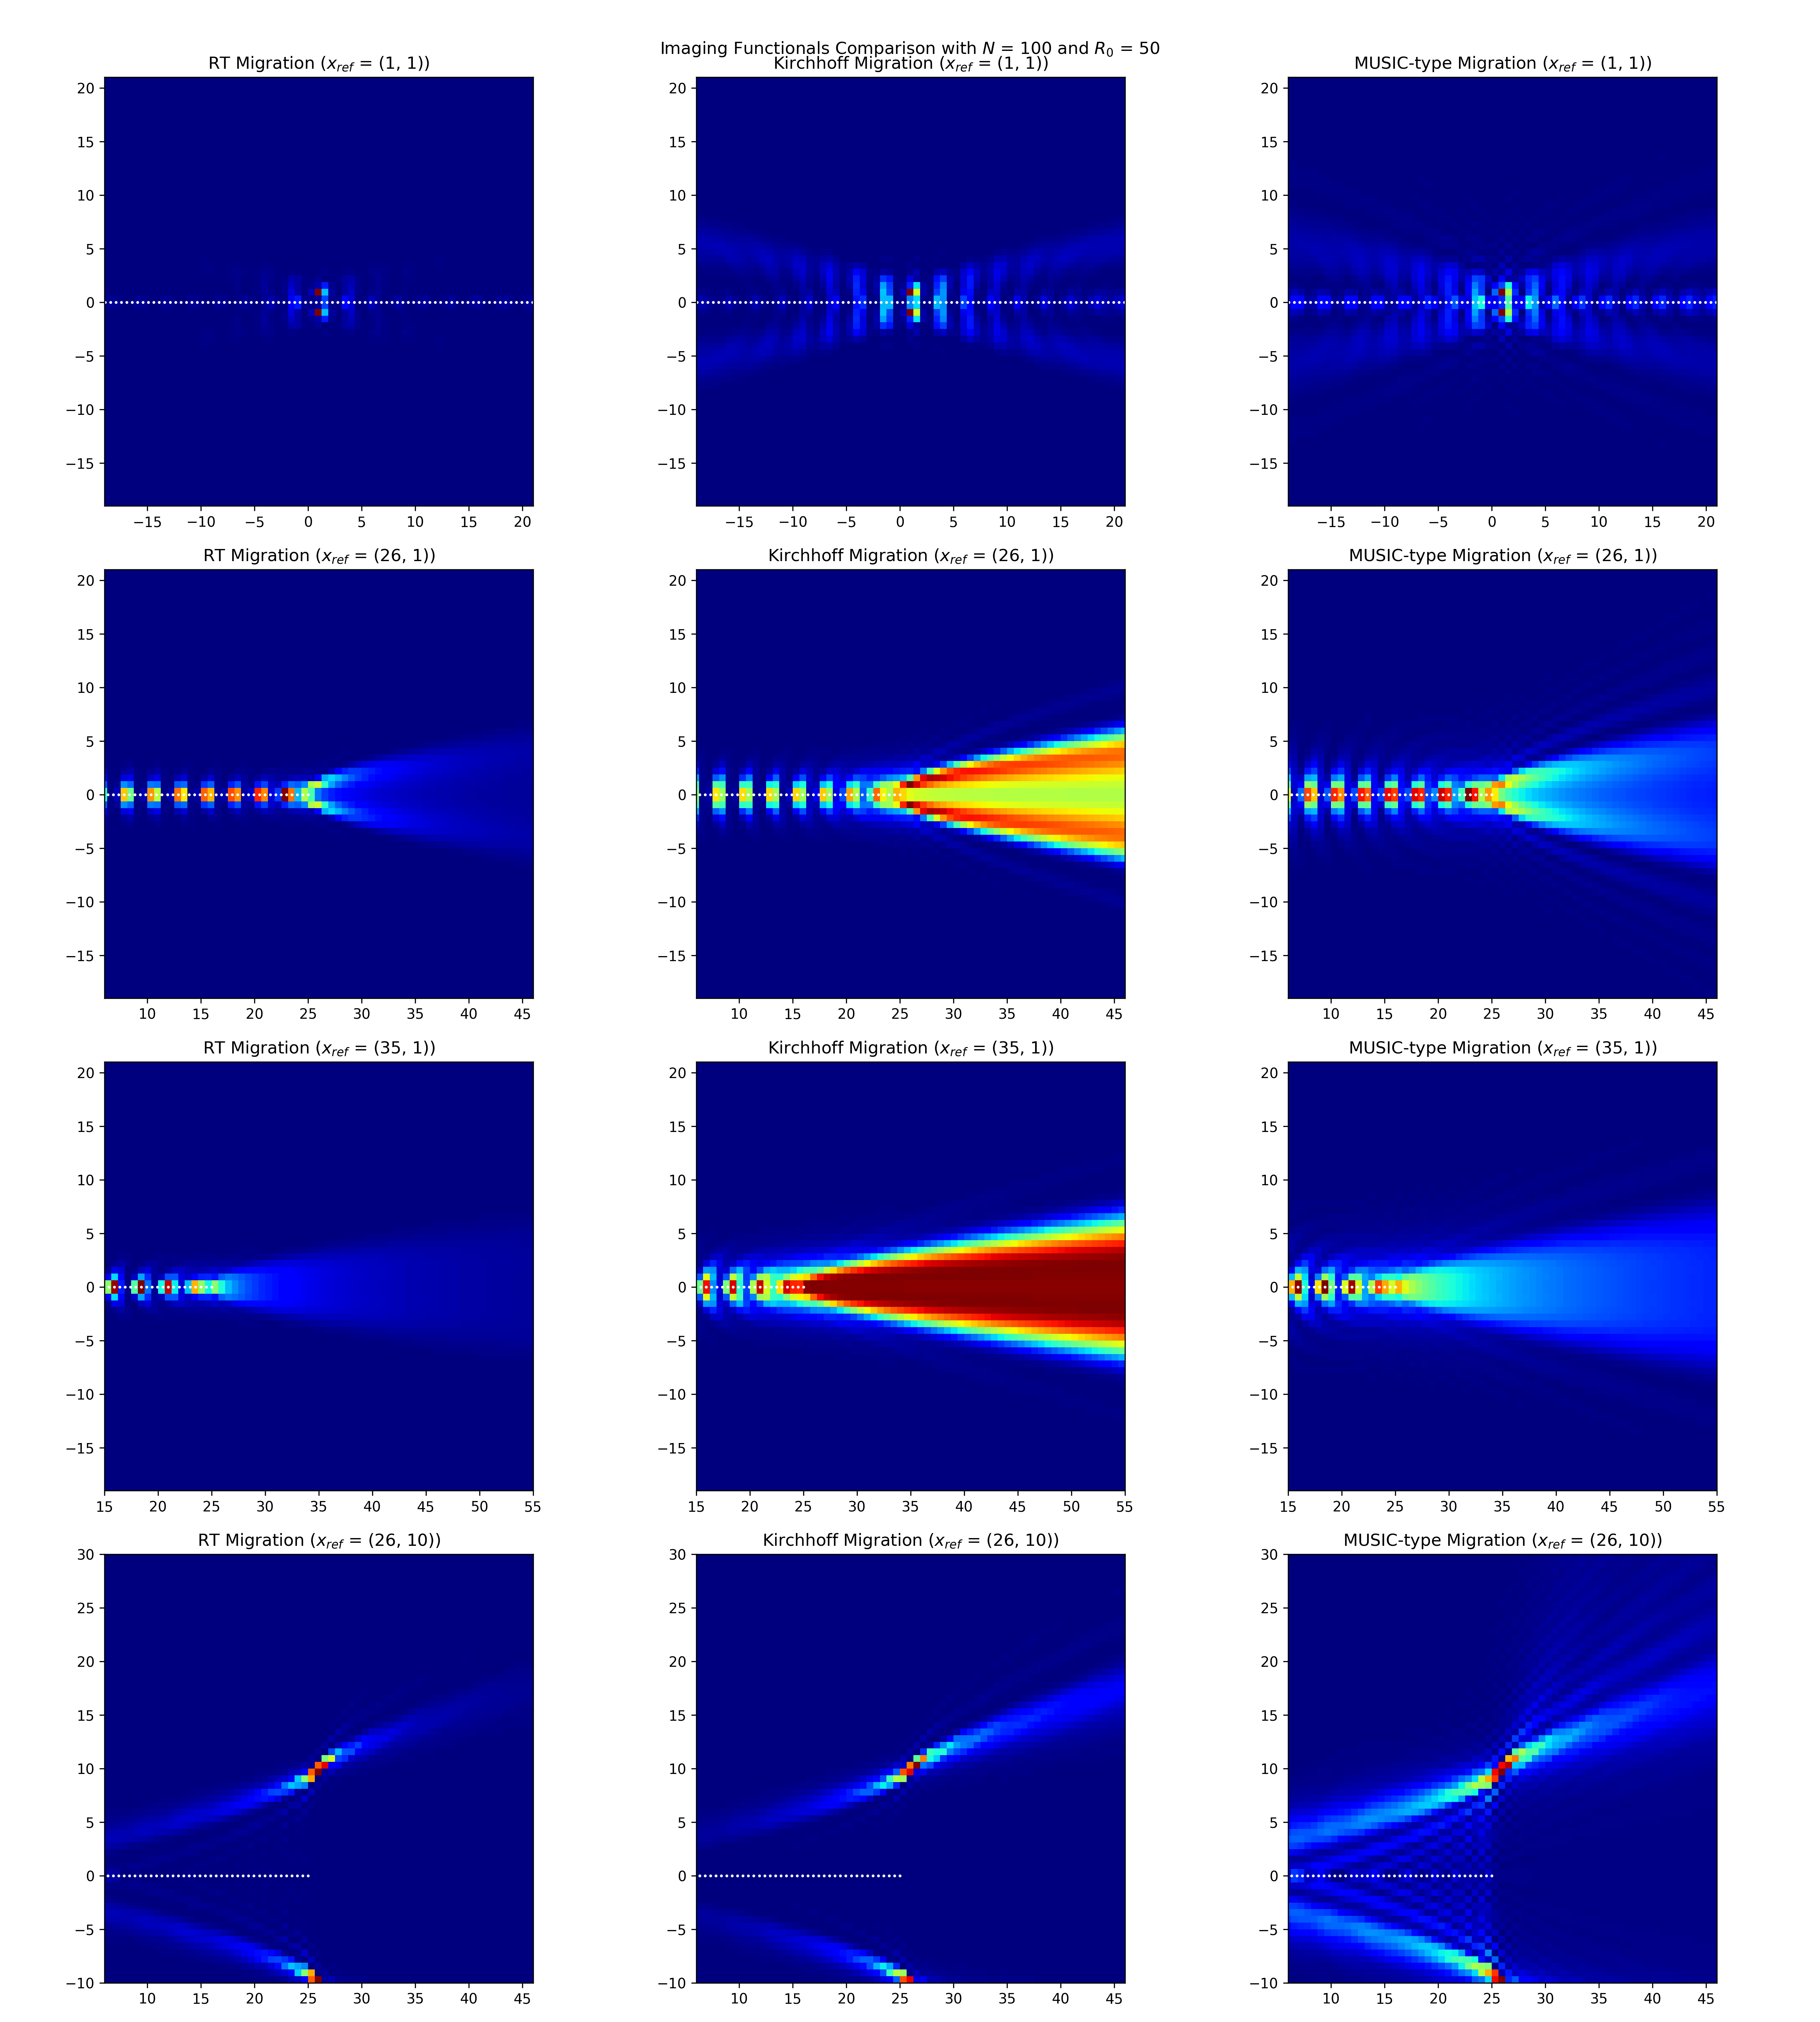
\includegraphics[width=\textwidth]{Partial_Aperture_Multiple_Reflectors.png}
    \end{center}
  \end{column}
  \begin{column}{0.44\textwidth}
    \begin{tcolorbox}[keybox, title=Effect of reflector distance]
      \footnotesize
      Moving the reflector \textbf{further from the array}:
      \begin{itemize}[leftmargin=0.5em, label=\textbullet]\setlength\itemsep{2pt}
        \item Increases the stand-off distance
        \item Degrades cross-range resolution
      \end{itemize}
    \end{tcolorbox}

    \vspace{0.1cm}
    \begin{tcolorbox}[stressbox]
      \scriptsize Focal spot characteristics scale with $|\bm{x}_{\mathrm{ref}}|$, in agreement with theoretical expressions for $r_c$ and $r_l$.
    \end{tcolorbox}
  \end{column}
  \end{columns}
\end{frame}


% ==============================================================================
% SECTION 5: RESULTS -- TIME-DEPENDENT (BROADBAND)
% ==============================================================================

\begin{frame}{Time-Dependent (Broadband) -- Partial Aperture}
  \footnotesize
  \vspace{-0.2cm}
  \begin{tcolorbox}[stressbox, title=Setup]
    \footnotesize $N\!=\!40$, $R_0\!=\!20$, broadband $\hat{f}(\omega) = \mathbf{1}_{[\omega_0-B,\,\omega_0+B]}(\omega)$, $\omega_0\!=\!2\pi$, $B\!=\!0.05\omega_0$, $\bm{x}_{\mathrm{ref}}\!=\!(0,100)$.
  \end{tcolorbox}

  \vspace{-0.4cm}
  \begin{columns}
  \begin{column}{0.54\textwidth}
    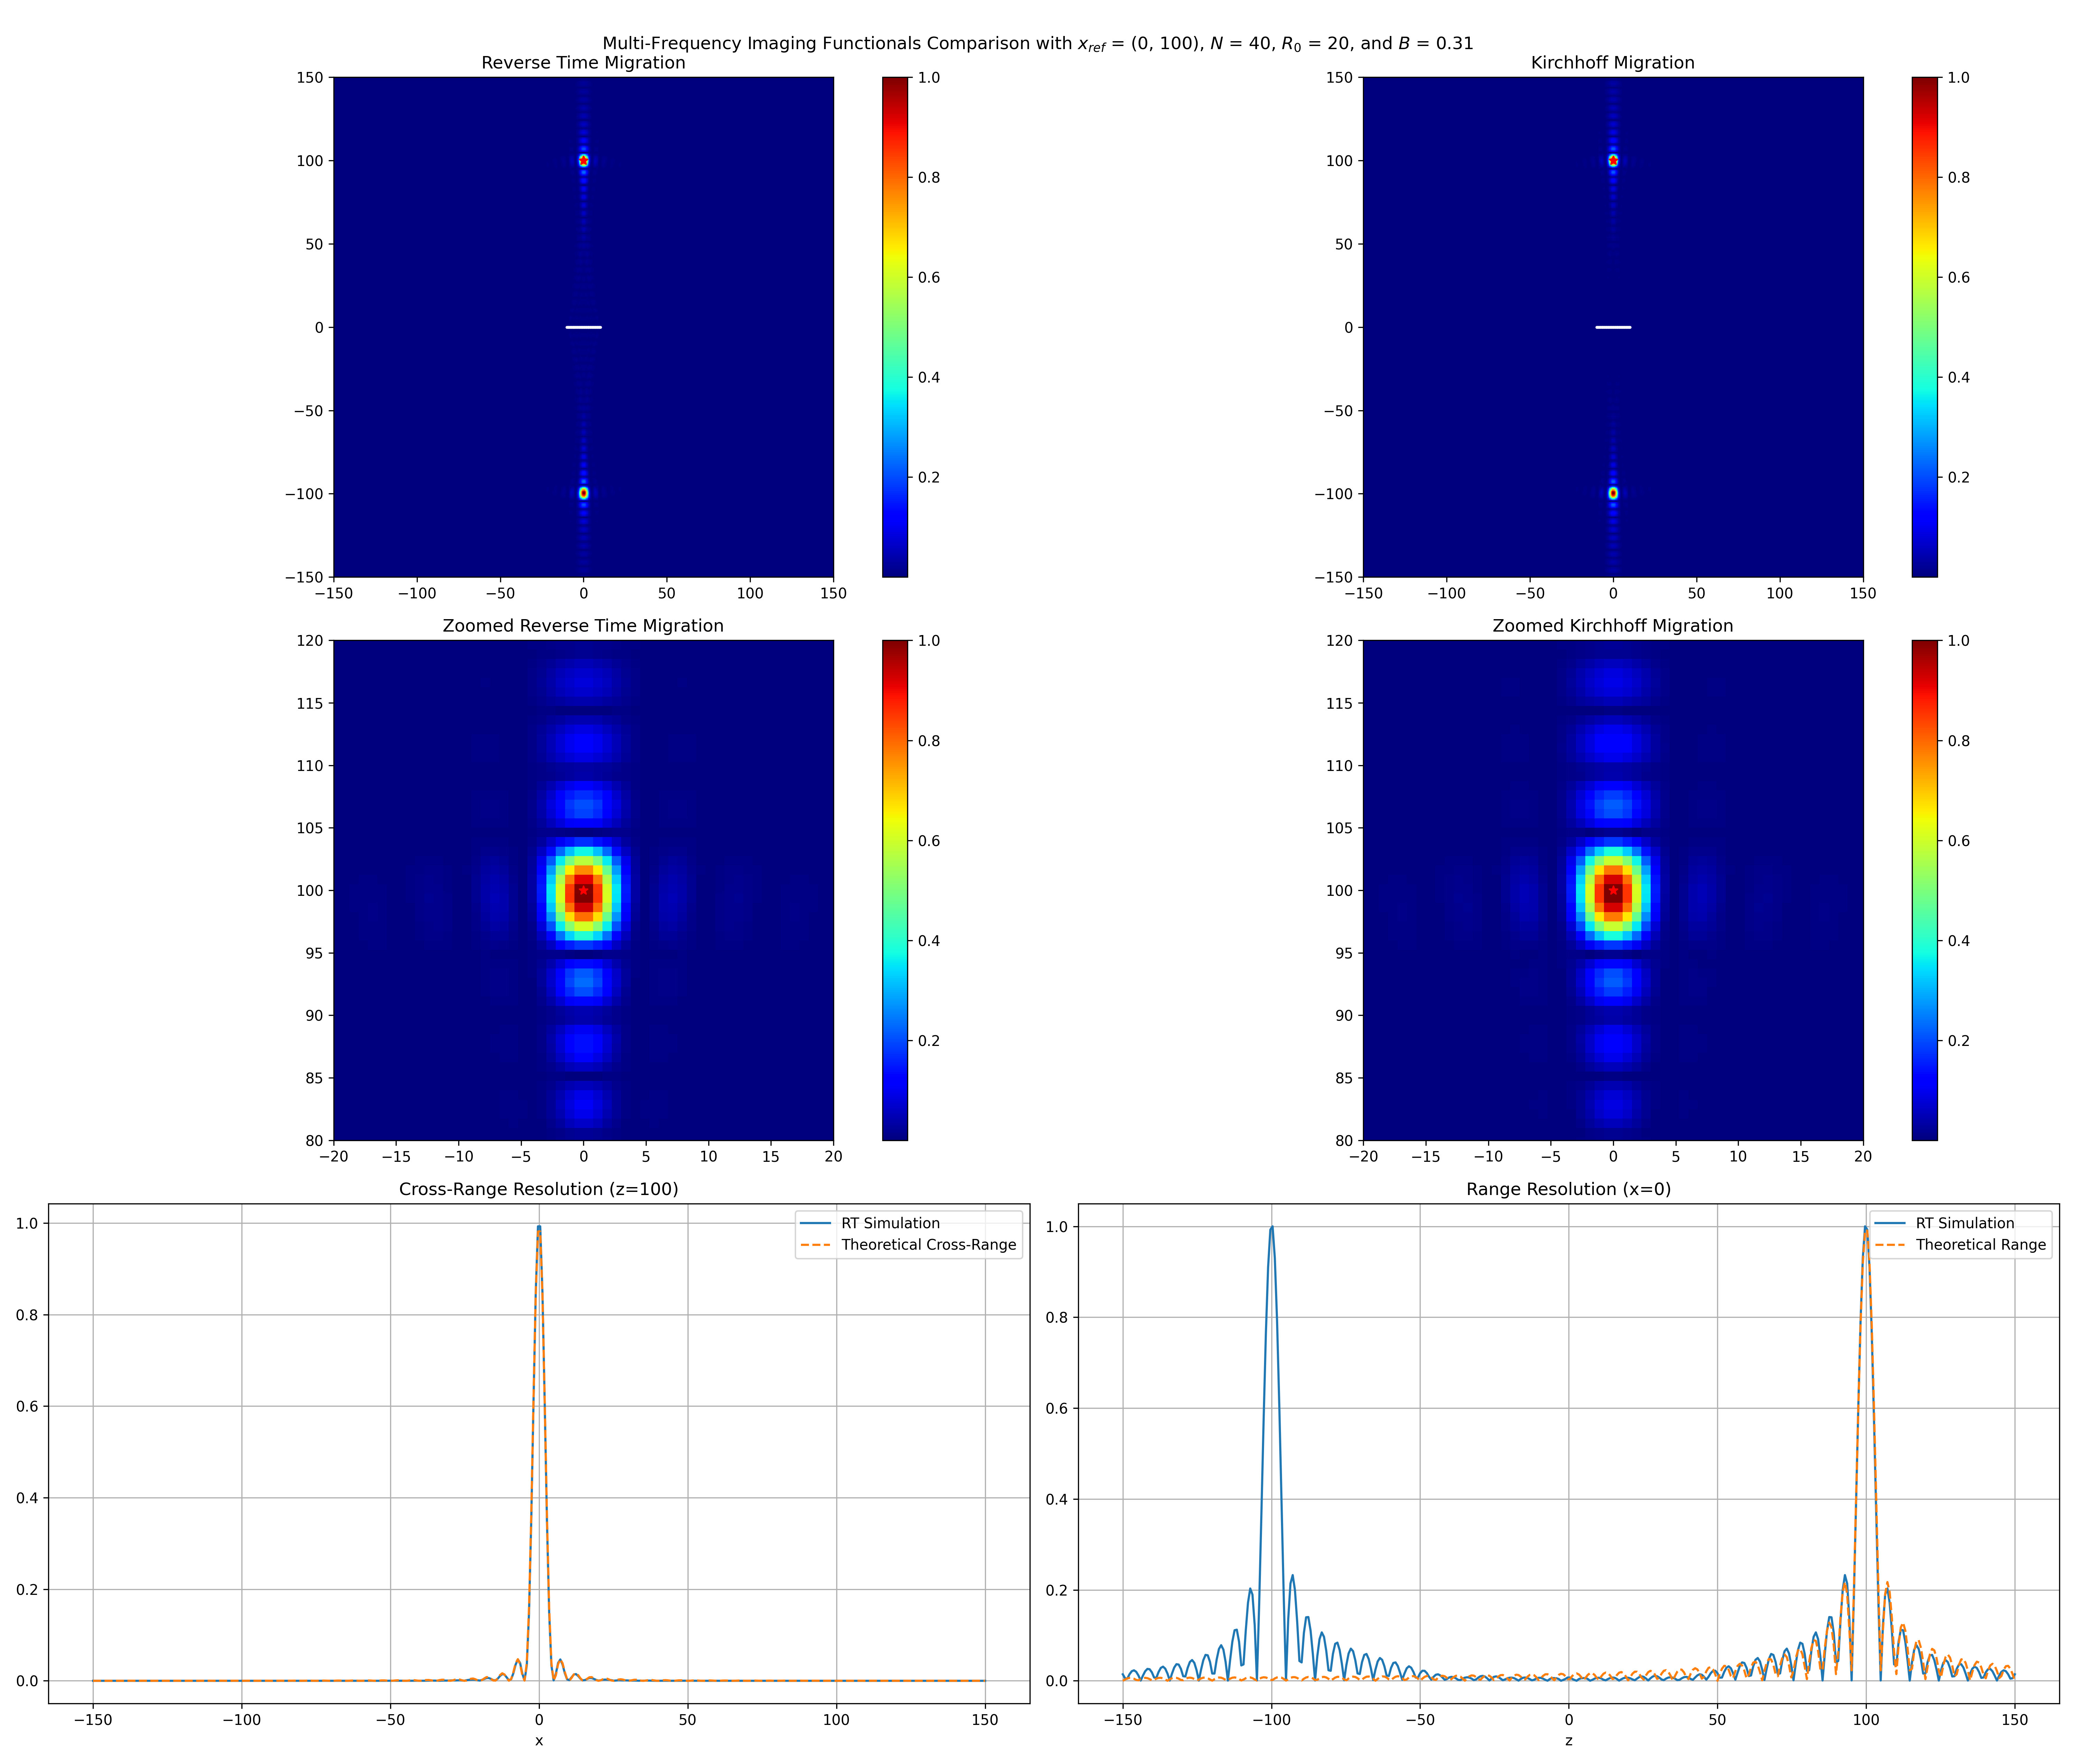
\includegraphics[width=\textwidth]{Time_Dependent.png}
  \end{column}
  \begin{column}{0.44\textwidth}
    \begin{tcolorbox}[keybox, title=Broadband advantage]
      \scriptsize
      \begin{itemize}[leftmargin=0.5em, label=\textbullet]\setlength\itemsep{2pt}
        \item Focal spot is \textbf{significantly more localized} than monochromatic.
        \item Cross-range: RT matches the $\operatorname{sinc}^2$ main peak and secondary lobes.
        \item Range: profile consistent with $|\operatorname{sinc}(2B|z-z_{\mathrm{ref}}|)|$ prediction.
      \end{itemize}
    \end{tcolorbox}

    \vspace{-0.3cm}
    \begin{tcolorbox}[resultbox]
      \scriptsize Broader frequency content $\Rightarrow$ improved coherent focusing in both directions.
    \end{tcolorbox}
  \end{column}
  \end{columns}
\end{frame}

\begin{frame}{Time-Dependent -- Influence of Bandwidth $B$}
  \small
  \vspace{-0.2cm}
  \begin{columns}
  \begin{column}{0.44\textwidth}
    \begin{center}
      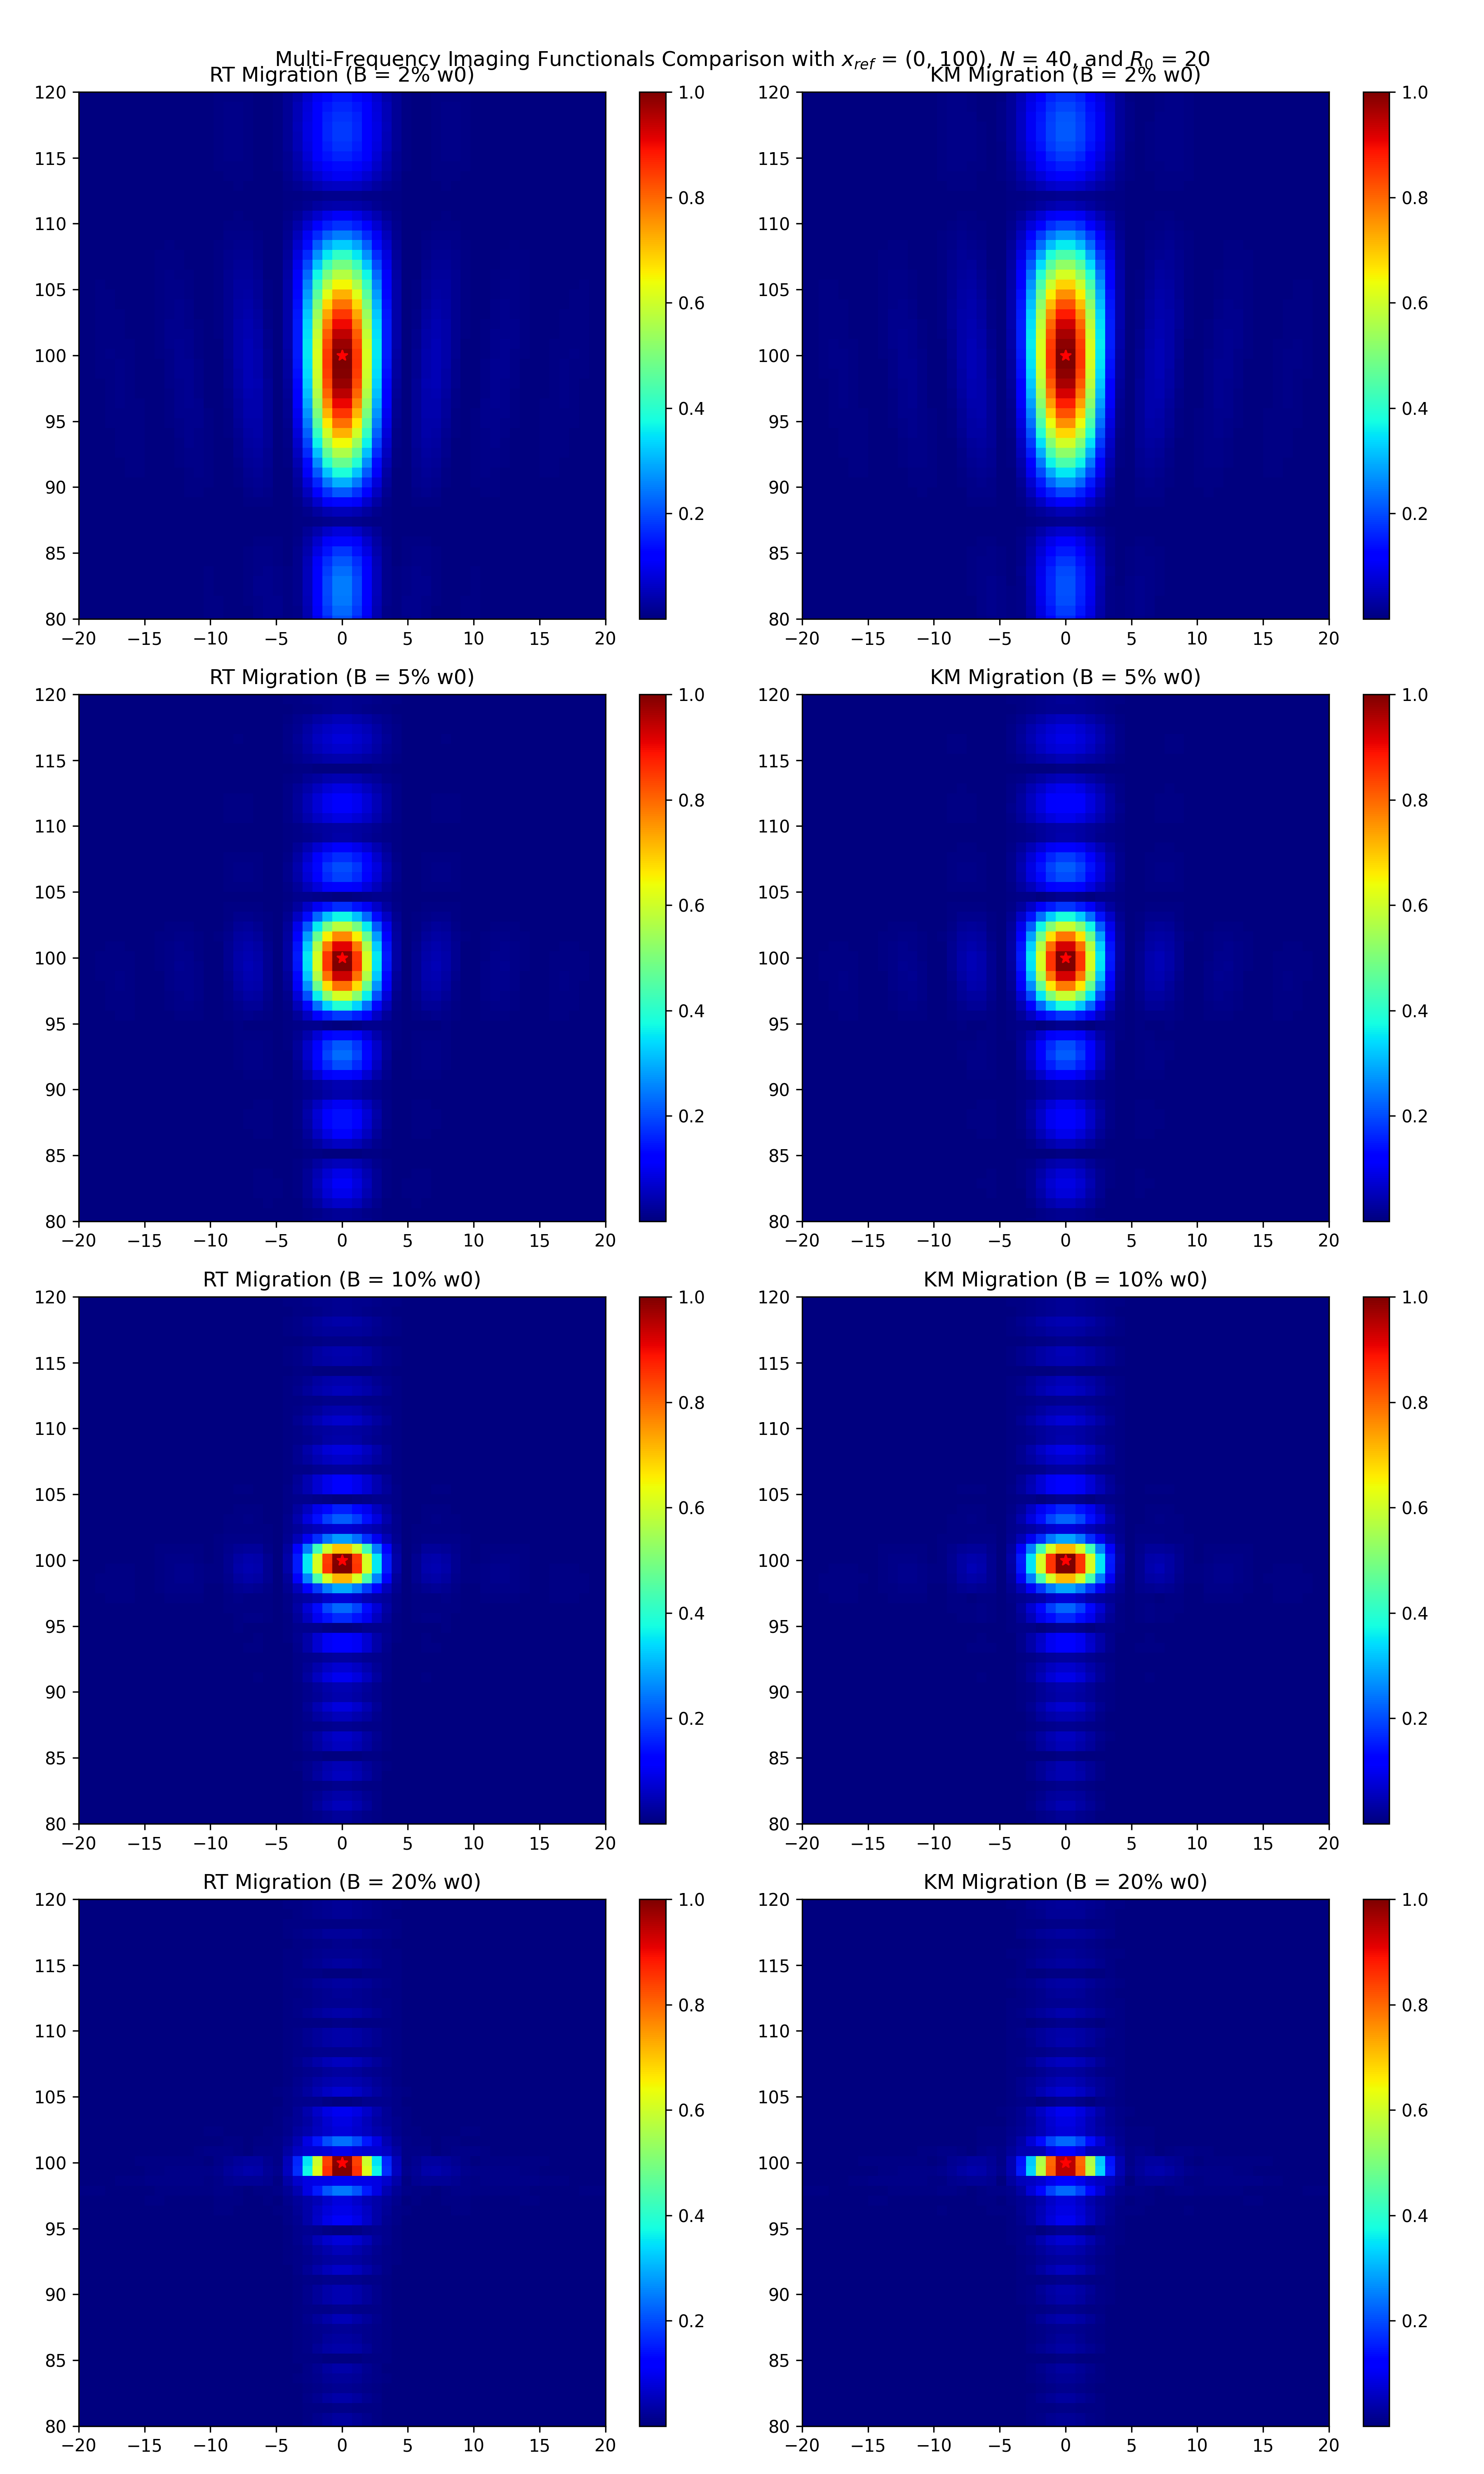
\includegraphics[width=0.82\textwidth]{Time_Dependent_Multiple_Bandwidths.png}
    \end{center}
  \end{column}
  \begin{column}{0.54\textwidth}
    \begin{tcolorbox}[keybox, title=Bandwidth vs.\ Resolution]
      \footnotesize
      \begin{itemize}[leftmargin=0.5em, label=\textbullet]\setlength\itemsep{3pt}
        \item \textbf{Range resolution:} $r_l \propto 1/B$
        \item \textbf{Cross-range resolution:} unchanged
      \end{itemize}
      Wider bandwidth $\Rightarrow$ sharper range profile.
    \end{tcolorbox}

    \vspace{0.1cm}
    \begin{tcolorbox}[resultbox]
      \scriptsize Increasing $B$ dramatically reduces range sidelobe level and sharpens the range profile, confirming the $\operatorname{sinc}$ dependence on bandwidth.
    \end{tcolorbox}
  \end{column}
  \end{columns}
\end{frame}


% ==============================================================================
% SECTION 6: STABILITY / NOISE
% ==============================================================================

\begin{frame}{Stability -- Noisy Model}
  \small
  \vspace{-0.2cm}
  \begin{tcolorbox}[keybox, title=Noise Model]
    The recorded signals are perturbed by complex Gaussian noise:
    \vspace{-0.15cm}
    $$\hat{u}_{rs}^{\mathrm{noisy}}(\omega) = \hat{u}_{rs}(\omega) + W_{rs}^{(1)}(\omega) + i\, W_{rs}^{(2)}(\omega)$$
    \vspace{-0.3cm}

    {\footnotesize where $W_{rs}^{(1)}, W_{rs}^{(2)} \sim \mathcal{N}(0,\, \sigma^2/2)$ i.i.d.}
  \end{tcolorbox}

  \vspace{-0.1cm}
  \noindent
  \begin{minipage}[t]{0.32\textwidth}
    \begin{tcolorbox}[stressbox, title=Full aperture, halign=center]
      \footnotesize RT \& KM
    \end{tcolorbox}
  \end{minipage}
  \hfill
  \begin{minipage}[t]{0.32\textwidth}
    \begin{tcolorbox}[stressbox, title=Partial aperture, halign=center]
      \footnotesize RT, KM \& MUSIC
    \end{tcolorbox}
  \end{minipage}
  \hfill
  \begin{minipage}[t]{0.32\textwidth}
    \begin{tcolorbox}[stressbox, title=Broadband, halign=center]
      \footnotesize RT \& KM
    \end{tcolorbox}
  \end{minipage}

  \begin{tcolorbox}[warnbox, title=Analysis strategy]
    \footnotesize
    For each configuration: images at increasing $\sigma$, then quantify localization error via \textbf{Monte Carlo simulation} (multiple noise realizations).
  \end{tcolorbox}

  \vspace{0.05cm}
  \begin{tcolorbox}[stressbox]
    \scriptsize \textbf{Note on MUSIC:} we use the noise-subspace variant $\mathcal{I}_{MU}(\bm{x}) = 1/(1-|\langle\hat{g},v_1\rangle|^2)$ to expose its super resolution behaviour and sensitivity to noise.
  \end{tcolorbox}
\end{frame}

\begin{frame}{Stability -- Full Aperture under Noise}
  \small
  \vspace{-0.2cm}
  \begin{center}
    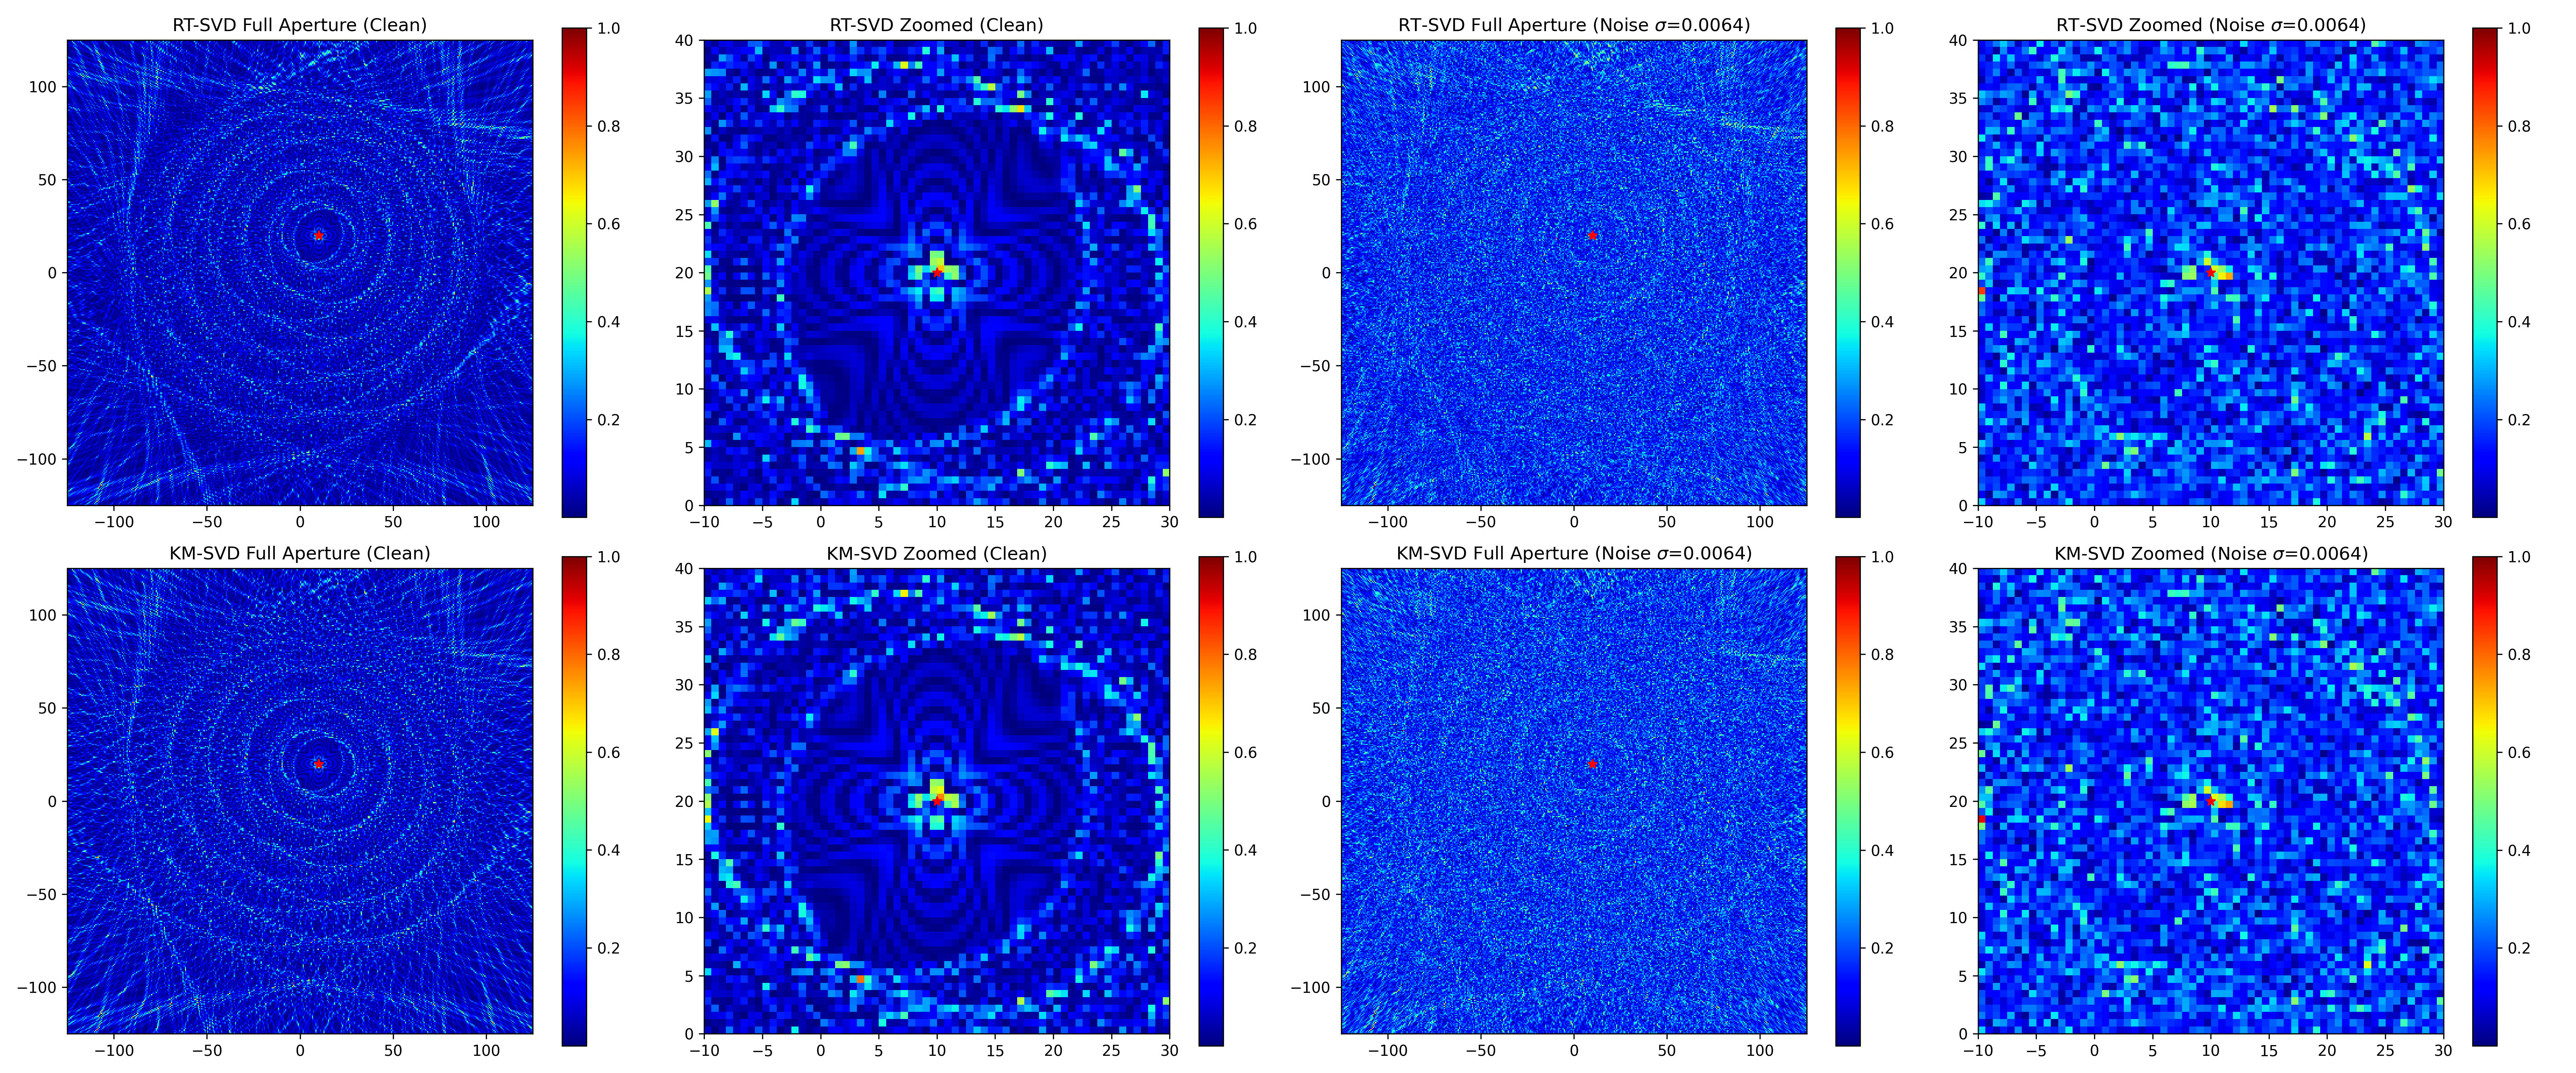
\includegraphics[width=\textwidth]{Noise_Full_Aperture_short.png}
  \end{center}

  \vspace{-0.2cm}
  \begin{tcolorbox}[resultbox, title=Result]
    \footnotesize RT and KM both manage to \textbf{handle noise} as $\sigma$ increases. Coherent integration over many transducer pairs provides a natural averaging effect that partially mitigates noise.
  \end{tcolorbox}
\end{frame}

 
\begin{frame}{Stability -- Time-Dependent Broadband under Noise}
  \small
  \vspace{-0.2cm}
  \begin{center}
    \includegraphics[width=\textwidth]{Noise_Time_Dependent_short.png}
  \end{center}

  \vspace{-0.2cm}
  \begin{tcolorbox}[resultbox]
    \footnotesize The broadband RT functional retains a \textbf{well-defined peak} even at elevated noise levels, benefiting from frequency diversity in addition to spatial averaging.
  \end{tcolorbox}
\end{frame}

\begin{frame}{Stability -- Partial Aperture under Noise}
  \small
  \vspace{-0.2cm}
  \begin{center}
    \includegraphics[width=0.9\textwidth]{Noise_Partial_Aperture_short.png}
  \end{center}

  \vspace{-0.2cm} 
  \noindent
  \begin{minipage}[t]{0.48\textwidth}
    \begin{tcolorbox}[resultbox]
      \scriptsize RT and KM remain \textbf{robust} for moderate noise levels.
    \end{tcolorbox}
  \end{minipage}
  \hfill
  \begin{minipage}[t]{0.48\textwidth}
    \begin{tcolorbox}[warnbox]
      \scriptsize MUSIC is sharper at low noise but \textbf{degrades abruptly} once $v_1$ is perturbed.
    \end{tcolorbox}
  \end{minipage}
\end{frame}


\begin{frame}{Stability -- Monte Carlo Analysis: RT vs.\ MUSIC}
  \footnotesize
  \vspace{-0.2cm}
  \begin{tcolorbox}[stressbox, title=RMSE of localization vs.\ noise level $\sigma$ (partial aperture)]
    \scriptsize Multiple noise realizations are generated for each $\sigma$ with Monte Carlo simulation. 
  \end{tcolorbox}

  \vspace{-0.3cm}
  \begin{columns}
  \begin{column}{0.48\textwidth}
    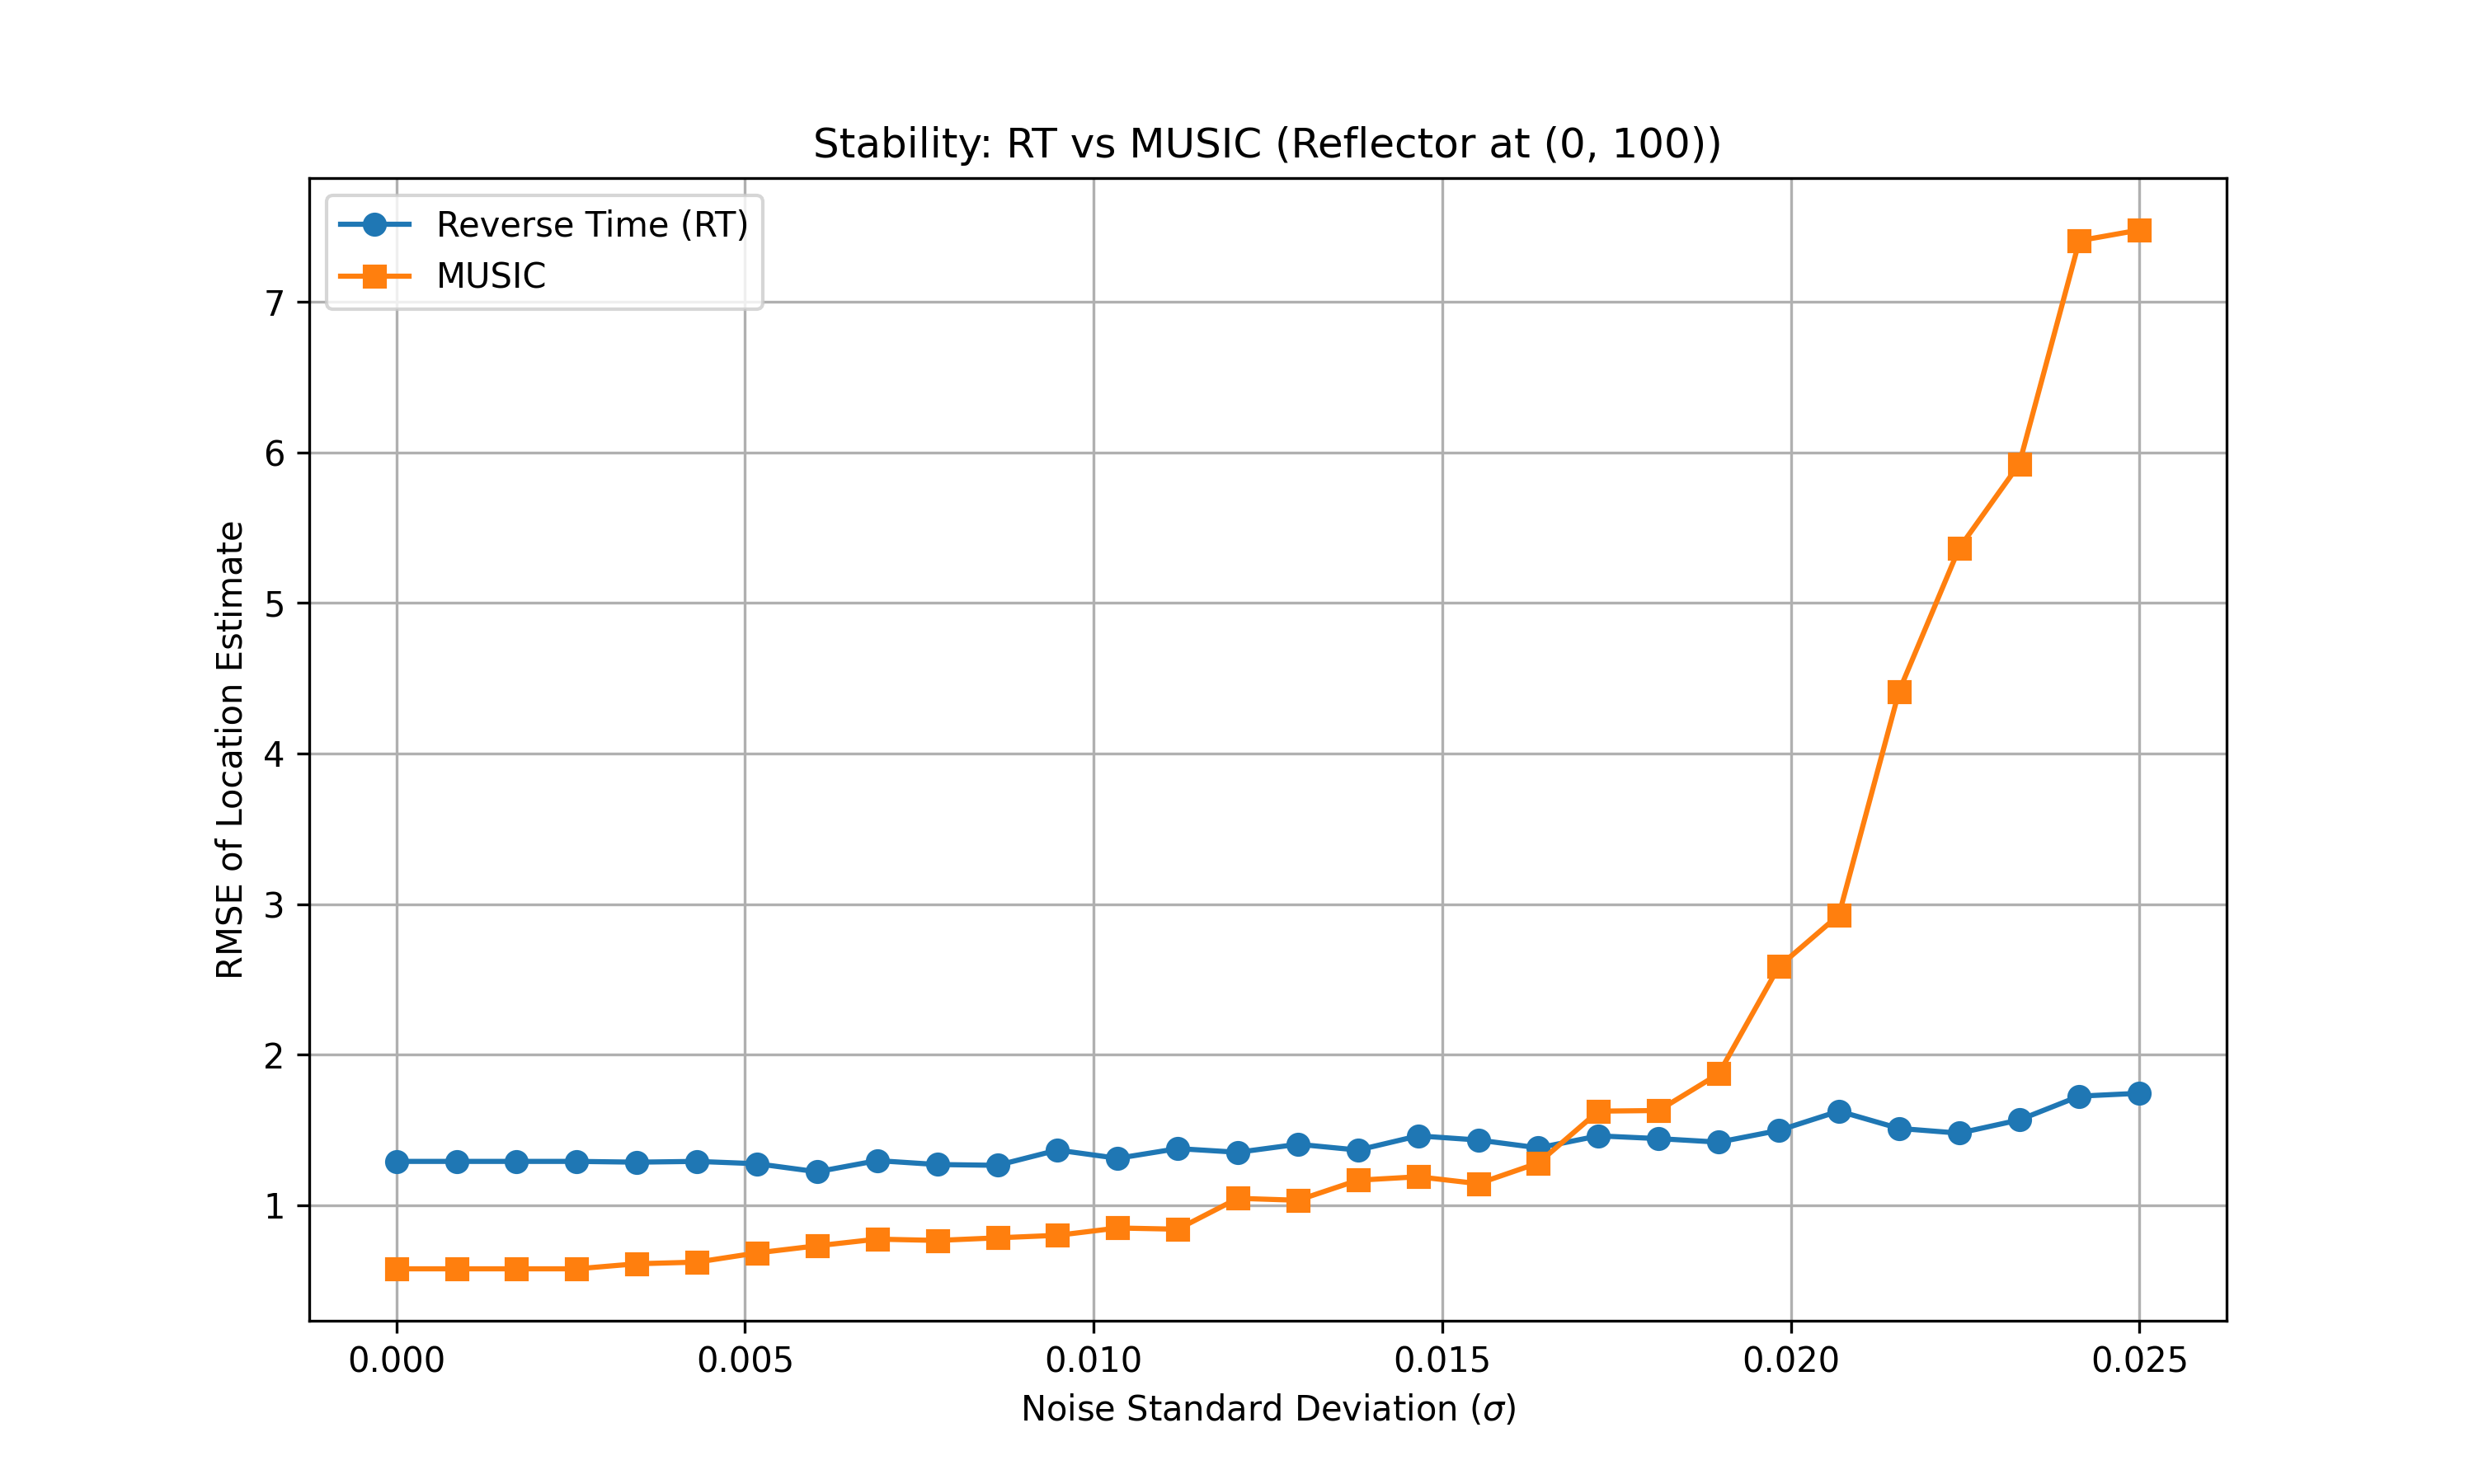
\includegraphics[width=\textwidth]{Stability_vs_Noise.png}
  \end{column}
  \begin{column}{0.50\textwidth}
    \begin{tcolorbox}[resultbox, title=RT: noise robustness]
      \scriptsize Localization error grows \textbf{slowly and steadily} with $\sigma$. Coherent back-propagation integrates over all source--receiver pairs, averaging out random noise.
    \end{tcolorbox}

    \vspace{-0.3cm}
    \begin{tcolorbox}[warnbox, title=MUSIC: noise fragility]
      \scriptsize Error remains very low for small $\sigma$, then \textbf{rises sharply} beyond a threshold. Once noise corrupts $v_1$, the functional fails abruptly.
    \end{tcolorbox}
  \end{column}
  \end{columns}

  \vspace{0.05cm}
  \begin{tcolorbox}[keybox]
    \footnotesize RT is more \textbf{robust}; MUSIC offers higher precision at low noise but is \textbf{fragile}.
  \end{tcolorbox}
\end{frame}


% ==============================================================================
% SECTION 7: CONCLUSION
% ==============================================================================

\begin{frame}{Conclusion}
  \scriptsize
  \vspace{-0.1cm}
  \begin{tcolorbox}[keybox, title=Summary of Findings, top=2pt, bottom=2pt]
    \begin{itemize}[leftmargin=0.5em, label=\textbullet]\setlength\itemsep{1.5pt}
      \item \textbf{Full aperture:} RT and KM agree closely; both approach theoretical $J_0^2$ spot as $R_0,N\!\to\!\infty$.
      \item \textbf{Partial aperture:} linear geometry $\Rightarrow$ mirror artifact in range; cross-range resolution $r_c\!=\!\lambda|x_{\mathrm{ref}}|/R_0$. MUSIC provides sharper image.
      \item \textbf{Broadband:} increased bandwidth drastically improves range resolution ($r_l \!\propto\! 1/B$), consistent with $\operatorname{sinc}$ theory.
      \item \textbf{Noise:} RT degrades only in full aperture. MUSIC is precision-first but collapses beyond a noise threshold. Computing with SVD seems less sensitive to noise.
    \end{itemize} 
  \end{tcolorbox}
 

  \begin{tcolorbox}[warnbox, title=Perspectives, top=2pt, bottom=2pt]
    \begin{itemize}[leftmargin=0.5em, label=\textbullet]\setlength\itemsep{1.5pt}
      \item Extension to heterogeneous, anisotropic and even random media
      \item Advanced regularization to stabilize MUSIC at high noise (e.g., diagonal loading, eigenvalue thresholding, use broadband data, etc.)
      \item Multiple reflectors and mutual interference
    \end{itemize}
  \end{tcolorbox}


  \begin{tcolorbox}[keybox, top=2pt, bottom=2pt]
    \textbf{Key take-away:} Array geometry, bandwidth, and noise level are the \textbf{three dominant factors} controlling resolution and stability of RT/KM imaging functionals.
  \end{tcolorbox}
\end{frame}


% ==============================================================================
% BIBLIOGRAPHY
%  ==============================================================================
\begingroup
\setbeamertemplate{footline}{}

\begin{frame}[allowframebreaks]{Bibliography}
\frametitle{Bibliography}
Ammari et al., \textit{Mathematical and Statistical Methods for Multistatic Imaging}, Springer, 2013.
\end{frame}
\endgroup

\end{document}